\documentclass[11pt,a4paper]{article}

% ---------------- packages ----------------
\usepackage[T1]{fontenc}
\usepackage{amsmath}
\usepackage{newtxtext,newtxmath}
\usepackage[margin=2.5cm,headheight=14pt]{geometry}
\usepackage{setspace}
\setstretch{1.12}
\usepackage{microtype}
\usepackage{booktabs}
\usepackage{array}
\usepackage{tabularx}
\usepackage{longtable}
\usepackage{xltabular}
\usepackage{pdflscape}
\usepackage{graphicx}
\usepackage{xcolor}
\usepackage{enumitem}
\usepackage{titlesec}
\usepackage{fancyhdr}
\usepackage[font=small,labelfont=bf,skip=6pt]{caption}
\usepackage{tikz}
\usetikzlibrary{positioning,arrows.meta,fit,backgrounds,calc}
\usepackage{placeins}
\usepackage{url}
\usepackage{hyperref}

\hypersetup{
  colorlinks=true,
  linkcolor=black,
  urlcolor=blue!55!black,
  pdftitle={Verified Optimization Agents: Phase 1},
  pdfauthor={Mushahid Hussain, Muhammad Waqas, Abdul Rauf},
}

% ---------------- layout ----------------
\titleformat{\section}{\Large\bfseries}{\thesection}{0.6em}{}
\titleformat{\subsection}{\large\bfseries}{\thesubsection}{0.6em}{}
\titleformat{\subsubsection}{\normalsize\bfseries}{\thesubsubsection}{0.6em}{}
\titlespacing*{\section}{0pt}{14pt}{8pt}
\titlespacing*{\subsection}{0pt}{12pt}{6pt}
\titlespacing*{\subsubsection}{0pt}{10pt}{4pt}

\pagestyle{fancy}
\fancyhf{}
\fancyhead[L]{\small AI4015 Agentic AI, Fall 2026}
\fancyhead[R]{\small Phase 1, Project G1-01}
\fancyfoot[C]{\small\thepage}
\renewcommand{\headrulewidth}{0.4pt}

\setlist{itemsep=2pt,topsep=4pt,parsep=0pt}
\setlength{\parskip}{4pt}
\setlength{\parindent}{0pt}
\renewcommand{\arraystretch}{1.18}
\widowpenalty=10000
\clubpenalty=10000
\displaywidowpenalty=10000

\newcolumntype{P}[1]{>{\raggedright\arraybackslash}p{#1}}
\newcolumntype{Y}{>{\raggedright\arraybackslash}X}

\definecolor{gapone}{RGB}{0,84,166}
\definecolor{gaptwo}{RGB}{196,82,0}
\definecolor{gapthree}{RGB}{0,122,61}
\newcommand{\gaptag}[2]{\textcolor{#1}{\textbf{[#2]}}}
\newcommand{\elem}[1]{\par\noindent\textbf{#1.}~}

% float placement: allow fuller pages and stack float pages from the top
\renewcommand{\topfraction}{0.9}
\renewcommand{\bottomfraction}{0.8}
\renewcommand{\textfraction}{0.07}
\renewcommand{\floatpagefraction}{0.85}
\setcounter{topnumber}{3}
\setcounter{totalnumber}{5}
\makeatletter
\setlength{\@fptop}{0pt}
\setlength{\@fpsep}{14pt}
\setlength{\@fpbot}{0pt plus 1fil}
\makeatother
\newcommand{\cthree}{C$^3$-Bench}

\begin{document}

% =====================================================================
% TITLE PAGE
% =====================================================================
\hypersetup{pageanchor=false}
\begin{titlepage}
\centering
\vspace*{0.6cm}
{\large\bfseries FAST National University of Computer and Emerging Sciences\par}
\vspace{1mm}
{\normalsize Islamabad Campus\par}
\vspace{1mm}
{\normalsize Department of Computer Sciences\par}
\vspace{10mm}
{\large AI4015 Agentic Artificial Intelligence, Fall 2026\par}
\vspace{1mm}
{\normalsize Semester Project, Phase 1: Literature Review, Proposal and Baseline\par}
\vspace{14mm}
\rule{\textwidth}{0.8pt}\par
\vspace{5mm}
{\LARGE\bfseries Verified Optimization Agents\par}
\vspace{3mm}
{\Large Requirement-Level Verification and Calibrated Abstention\\[1mm]for LLM-Based Optimization Modeling\par}
\vspace{5mm}
\rule{\textwidth}{0.8pt}\par
\vspace{8mm}
{\normalsize\textbf{Selected seed (G1-01):} LLM Agents that Translate Natural Language\\into Verified Optimization Models\par}
\vspace{14mm}
\begin{tabular}{l l l}
\toprule
\textbf{Name} & \textbf{Roll Number} & \textbf{Role}\\
\midrule
Mushahid Hussain & 23I-0541 & Group head\\
Muhammad Waqas & 23I-0569 & Member\\
Abdul Rauf & 23I-0591 & Member\\
\bottomrule
\end{tabular}\par
\vspace{14mm}
\begin{tabular}{r l}
\textbf{Supervisor:} & Muhammad Sajjad (G1 projects)\\
\textbf{Instructor:} & Muhammad Owais Idrees\\
\textbf{Repository:} & \url{https://github.com/mushi0541/verified-optimization-agents}\\
\textbf{Submitted:} & 17 October 2026\\
\end{tabular}
\vfill
\end{titlepage}
\hypersetup{pageanchor=true}

\begingroup
\setstretch{1.0}
\setlength{\parskip}{0pt}
\tableofcontents
\endgroup
\newpage

% =====================================================================
% 1. LITERATURE REVIEW AND RESEARCH GAPS
% =====================================================================
\section{Literature Review and Research Gaps}
\label{sec:lit}

This review covers ten peer-reviewed papers from 2025 and 2026 on using large language models (LLMs) to turn natural-language problem descriptions into optimization models that a solver can run. Four papers appeared at the International Conference on Machine Learning (ICML) 2026~[1], [2], [3], [4], two at the Conference on Neural Information Processing Systems (NeurIPS) 2025~[5], [6], one at ICML 2025~[7], two at the International Conference on Learning Representations (ICLR) 2025~[8], [9], and one in the journal \textit{Operations Research} in 2025~[10]. We found the ten papers through keyword searches of arXiv, OpenReview and conference proceedings, and confirmed each paper's venue and year on its official proceedings or publisher page. ICML, NeurIPS and ICLR are all ranked A* in the ICORE2026 conference ranking (the CORE ranking, now run as an international collaboration called ICORE). Four further works are cited as supporting evidence but are not counted among the ten: a benchmark audit~[11] and three recent papers close to our gaps~[12], [13], [14], of which only~[12] has been peer-reviewed so far. Sections~\ref{sec:base} to~\ref{sec:gaps} analyze the base paper, summarize the other nine papers, compare all ten and derive the three research gaps.

% ---------------------------------------------------------------------
\subsection{Base Paper Selection and Validation}
\label{sec:base}

\subsubsection{Full Reference and Ranking Proof}

Y.~Chen, C.~Cheng, Y.~Sun, Z.~Ling, and D.~Ge, ``OPT-Engine: Benchmarking the limits of LLMs in optimization modeling via complexity scaling,'' in \textit{Proc.\ 43rd Int.\ Conf.\ Mach.\ Learn.\ (ICML)}, Seoul, South Korea, Jul.\ 2026, vol.~306, pp.~13807--13834~[1].

The paper is published in the ICML 2026 proceedings (Proceedings of Machine Learning Research, volume 306). ICML is ranked \textbf{A*} in ICORE2026, as shown in Figure~\ref{fig:core-rank}, so the base paper meets the requirement of a paper published in 2025 or 2026 at an A*/A-ranked conference.

\begin{figure}[htbp]
\centering
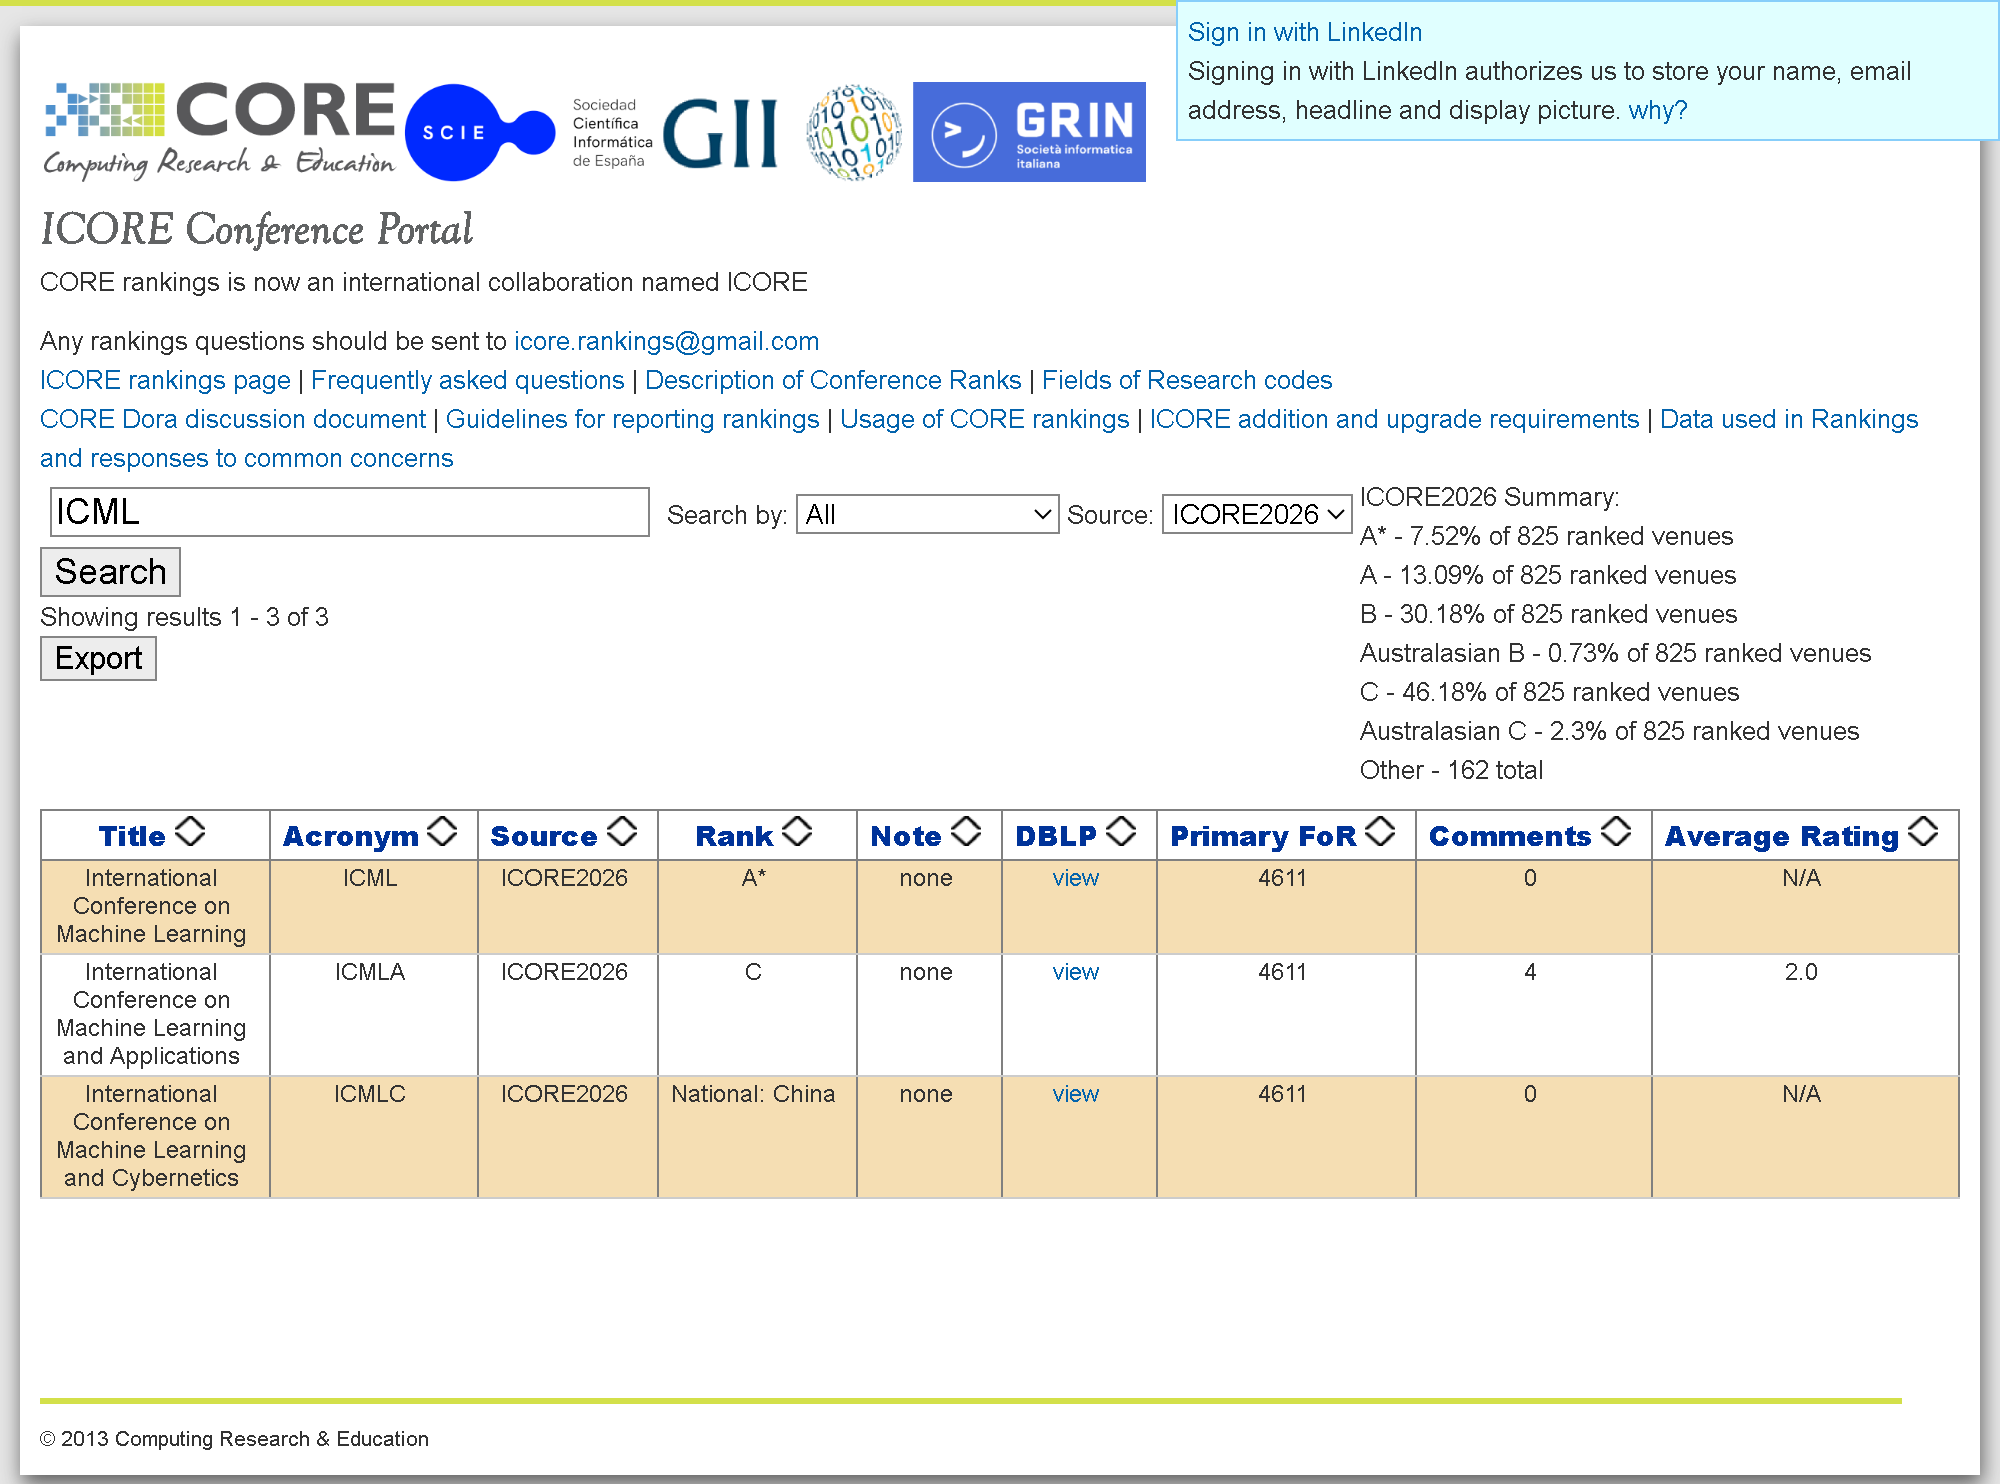
\includegraphics[width=0.92\textwidth]{ICML-ICORE2026-ranking.png}
\caption{Ranking proof for the base paper venue. ICML is ranked A* in ICORE2026 (\mbox{portal.core.edu.au}, accessed 17 October 2026).}
\label{fig:core-rank}
\end{figure}

\subsubsection{Justification for Selection}

We selected OPT-Engine for four reasons.
\begin{enumerate}[leftmargin=1.6em]
\item \textbf{Same task.} It studies exactly the task of our seed: an LLM reads an optimization question in plain language, writes a model, and a solver computes the answer. Its Solver-Integrated Reasoning (SIR) setting is the natural single-agent baseline for our system.
\item \textbf{Reliable, controlled data.} Its problems are produced by generators that compute exact reference optima. Size parameters control the complexity of each of its ten problem classes, and the data are released together with the evaluation scripts. This reduces the labeling errors reported for several older benchmarks (Section~\ref{sec:summaries}).
\item \textbf{Fit with all three gaps.} Its linguistic perturbation set provides reworded questions for paraphrase checks (Gap~1), its ten classes allow leave-one-class-out tests of a refusal rule (Gap~2), and its comparison of reasoning paradigms without matched token budgets motivates an equal-budget study (Gap~3).
\item \textbf{Reproducible comparison.} We can run its SIR setting with a free open model, using PuLP and HiGHS in place of Gurobi, so our results can be compared with it on the same data and metric.
\end{enumerate}

\subsubsection{Core Problem}

Existing benchmarks for LLM-based optimization modeling are fixed collections of mostly textbook-style problems. They do not allow problem size or difficulty to be changed in a controlled way. As a result, it is unclear at what level of complexity LLMs start to fail, and whether the failures come from reasoning, arithmetic or the formulation of constraints. OPT-Engine studies three questions: whether pure-text reasoning stays reliable as problems grow, whether external computational tools can make up for its arithmetic weaknesses and what limits the solver-integrated approach.

\subsubsection{Agent Architecture}

OPT-Engine is a benchmark paper and does not propose a multi-agent system. It compares three single-agent reasoning paradigms that differ in the tools given to the LLM:
\begin{itemize}[leftmargin=1.6em]
\item \textbf{Pure-Text Reasoning (PTR):} the LLM reasons step by step in text and states the final answer, with no code execution.
\item \textbf{Computational PTR (CompPTR):} the LLM may run Python with computational libraries such as scipy, but has no global optimization solver.
\item \textbf{Solver-Integrated Reasoning (SIR):} the LLM writes a model in code, and an exact solver (for example Gurobi) computes the optimum. This is a single agent with one tool.
\end{itemize}
Four models are tested: DeepSeek-V3.2, GPT-5.1, Qwen3-4B-Instruct and Qwen3-4B-RL (a 4B model further trained with reinforcement learning from verifiable rewards).

\subsubsection{Datasets}

The data released with the paper, named \cthree{} (Controllable and Configurable Complexity Benchmark) in the authors' repository, are produced by parametric generators. A difficulty parameter, such as the number of cities in the traveling salesman problem (TSP), sets the complexity level of each instance, and a solver template computes its exact optimum. The ten problem classes are five linear programs (LP: Inventory, Portfolio, Production, Transportation and Pollution Control) and five mixed-integer programs (MIP: TSP, Knapsack, Bin Packing, Job-Shop Scheduling and Min-Cost Network Flow). Three perturbation sets test robustness on Inventory, Knapsack and TSP: \textit{linguistic complexity} (the same instance in easy, moderate and hard wording), \textit{objective perturbation} (a constant added to the objective, which leaves the optimal solution unchanged), and \textit{constraint augmentation} (a few extra constraints with no new variables). The release contains 1,810 canonical problems (from 50 to 620 per class) and 3,760 perturbation rows. The paper counts a prediction as correct when its relative error is below $10^{-3}$, averages accuracy over ten instances at each complexity level, and reports feasibility, optimality gap and execution rate for some settings.

\subsubsection{Key Results}

\begin{enumerate}[leftmargin=1.6em]
\item \textbf{Solvers remain necessary.} With DeepSeek-V3.2, on TSP at the Hard level, accuracy is 2.0\% with PTR, 44.0\% with CompPTR and 80.0\% with SIR. On Min-Cost Network Flow, PTR accuracy is 10.0\% at Easy and 0.0\% at Medium and Hard, while SIR reaches 100\% at every level. On Knapsack, PTR accuracy falls from 89.2\% to 45.6\% as difficulty rises, while SIR stays above 91\%.
\item \textbf{Constraint formulation is the main weakness.} Linguistic and objective perturbations leave accuracy roughly stable, but constraint augmentation causes a consistent accuracy drop for both PTR and SIR. The failure traces suggest that errors in the formulation, for example omitted constraints, pass through to the solver in SIR and lead to wrong objectives in PTR. The authors conclude that computational tools help with local calculations but do not make the model respect global constraints.
\item \textbf{Small models struggle to produce runnable code.} Qwen3-4B-Instruct produces executable code for only 23.1\% (TSP), 23.1\% (Knapsack) and 35.6\% (Inventory) of problems, against 86.4\%, 100\% and 88.8\% for DeepSeek-V3.2. Reinforcement learning helps: Qwen3-4B-RL outperforms PTR across the complexity dimensions.
\end{enumerate}

\subsubsection{Limitations}

\textbf{Stated by the authors.}
\begin{itemize}[leftmargin=1.6em]
\item Only exact-solution modeling is covered; for large NP-hard instances, exact models can be too slow, and heuristics are preferred.
\item Tracks that measure optimality gaps, run time and robustness under time limits, and that test whether LLMs can design or choose heuristics, are future work.
\item Only linear structures (LP and MIP) are included; nonlinear, stochastic and dynamic programs are left for future work.
\end{itemize}
\textbf{Identified by our group.}
\begin{itemize}[leftmargin=1.6em]
\item The paper measures failures but gives no way to detect them at run time: generated models are not verified, and there is no abstention, escalation or multi-agent design. An LLM judge is used only to validate the reworded benchmark text.
\item Accuracy is the main quality measure; feasibility, optimality gap and execution rate appear only for some settings. The paper does not report how often a wrong answer would be accepted, and gives no confidence intervals.
\item Token budgets are not matched across paradigms. The main results use one maximum response length of 16,128 tokens, but token use is not controlled, and in one reported case (TSP with DeepSeek-V3.2) PTR even uses fewer tokens near the size where its accuracy drops sharply, because it switches from enumeration to heuristics.
\item Only four models are tested, with a single small open model family.
\item The released classes are uneven in size (50 to 620 problems), and perturbations cover only three classes. The ten problem classes are textbook models wrapped in short scenario stories, not real multi-step operational workflows.
\item Results are reported per class, but nothing estimates how reliable a system is on a class it has not seen before, which is the setting a deployed refusal rule must face.
\end{itemize}

\subsubsection{How Our Project Builds On, Compares Against and Goes Beyond the Base Paper}

\textbf{Builds on.} We use \cthree{} and its perturbation sets as our main evaluation data, adopt its SIR setting as our baseline (with PuLP and HiGHS in place of Gurobi), and grade answers with the tolerance in its released evaluation code.

\textbf{Compares against.} We run the SIR setting with an open model (gpt-oss-120b) and compare it with our system on the same problems and metric, class by class. Every Phase~2 result will be reported next to this base-paper setting.

\textbf{Goes beyond.} (1) We add a verifier with label-free, requirement-level signals (Gap~1): \textit{number coverage}, the share of the numbers in the question that appear in the model code; \textit{requirement coverage} (added in Phase~2), the share of the requirements listed by our parser that the code implements as named constraints; and \textit{paraphrase-optimum agreement}, the share of independently solved rewordings of the question that reach the same optimum. (2) We add a decision layer that answers, abstains or escalates, with a threshold calibrated to a target \textit{wrong-accept rate} (the share of answered problems that are wrong) and tested on held-out problem classes (Gap~2). (3) We compare single-agent and multi-agent designs at equal token budgets (Gap~3). (4) We build OpsOR-Bench, a small set of operations problems generated from parameterized scenarios, as an extra test of distribution shift.

% ---------------------------------------------------------------------
\subsection{Critical Summaries of Nine Additional Papers}
\label{sec:summaries}

Each summary covers six elements: the problem, the method, the data, the results, the limitations (split into those stated by the authors and those identified by our group), and the relevance to this project.

\subsubsection[Opt-Verifier (ICML 2026)]{Opt-Verifier~[2] (ICML 2026)}

\elem{Problem} LLM-generated optimization models often miss implicit constraints, and running the code cannot reveal such formulation errors.
\elem{Method} A fixed multi-agent workflow distills the structure of the question to guide formulation, then checks the model from two sides: a structure-side evaluator compares an interpretation of the model with this structure, and a solution-side evaluator judges an explanation of the solver output. Each gives a binary verdict with a comment, and a refinement agent revises the model. The main comparison uses GPT-4o-mini; other backbones are also tested.
\elem{Data} NL4Opt (289 problems), MAMO ComplexLP (211), a 19-problem ComplexOR subset, IndustryOR (100) and OptMATH-Bench (166).
\elem{Results} Average solving accuracy is 64.3\%, against 50.6\% for OptiMUS and 46.6\% for Chain-of-Experts with the same backbone, at about 9 agent calls and 5,300 to 8,500 tokens per problem. On hard IndustryOR problems, the structure-side check has 83\% precision and 68\% recall.
\elem{Limitations} \textit{Stated by the authors:} none, as the paper has no limitations section. \textit{Identified by our group:} the verifiers are tested on 30 problems, with 270 wrong models made by deleting or rewriting parts of correct ones; verdicts are binary and uncalibrated, so they cannot support refusal at a known error rate; its structure check ignores numerical values; cost is compared only with multi-agent systems.
\elem{Relevance} Its precision and recall give a reference point for our verifier signals (Gap~1), and its token figures inform the equal-budget study (Gap~3).

\subsubsection[MIPLIB-NL (ICML 2026)]{MIPLIB-NL: Constructing an Industrial-Scale Benchmark~[3] (ICML 2026)}

\elem{Problem} Benchmarks hold small or synthetic problems, while industrial mixed-integer programs are far larger, so benchmark accuracy says little about practice.
\elem{Method} Experts recover indexed variable groups and constraint families from MIPLIB 2017 solver files and describe them in text. Several LLMs try to rebuild each model from the text and data alone (up to eight attempts each). Of 245 candidates, 163 passed and experts kept 60 of the other 82.
\elem{Data} MIPLIB-NL: 223 instances with text, data files, a model and code; 14 systems are scored by pass@1 (the first sample is correct) and pass@8 (at least one of eight samples is correct).
\elem{Results} The best system, GPT-5.1, solves 39.05\% (mean 17.85\%). SIRL-32B scores 87.40\% on MAMO-Complex but 1.43\% here, and OptMATH-7B 0.00\%. Failures are 48.3\% modeling errors, 45.0\% execution errors and 6.7\% timeouts.
\elem{Limitations} \textit{Stated by the authors:} they estimate that only about 40\% of MIPLIB 2017 could be converted; validation is existential, since one successful LLM reconstruction is enough; experts check the structure, not every detail; the data inherit the domain biases of MIPLIB 2017; the 8 infeasible and 15 open instances cannot be checked by solver matching and are not scored. \textit{Identified by our group:} it is a benchmark only, with no verifier, agentic baseline, token-cost measurement or refusal study.
\elem{Relevance} Fine-tuned models fail on these industrial problems, the shift a refusal rule must survive (Gap~2); omitted constraints motivate coverage checks (Gap~1).

\subsubsection[VeriSimpl (ICML 2026)]{VeriSimpl~[4] (ICML 2026)}

\elem{Problem} Generated optimization programs often run but do not implement the stated task, which execution alone cannot reveal.
\elem{Method} Up to ten sampled programs are checked with simplified solver queries. Each constraint is mutated three ways (satisfied with a margin, tight or violated), and the LLM judges from the text whether each version's solver witness is feasible; for variables, the solver fixes some optimal values and the LLM infers the rest. The best-scoring program is returned.
\elem{Data} NL4Opt (269 problems), NLP4LP (62), ComplexOR (17) and IndustryOR (96), with GPT-4o, DeepSeek-R1 and Mistral Large.
\elem{Results} With GPT-4o, average accuracy rises from 56.6\% to 65.5\% (SelfDebug: 59.1\%), and with DeepSeek-R1 from 62.5\% to 72.8\%. Fully verified GPT-4o programs are 91.5\% correct, but only 34.2\% of correct programs pass full verification (a recall the paper calls coverage); for DeepSeek-R1, 78.5\% precision at 23.0\% recall.
\elem{Limitations} \textit{Stated by the authors:} the queries cannot detect requirements that a program omits entirely, verification passes when the program and the LLM share a misreading, and recall is low. \textit{Identified by our group:} three test sets are small (17 to 96 problems), without confidence intervals; token cost is not reported; the precision-recall trade-off is not turned into a refusal rule.
\elem{Relevance} Its blind spot for omitted requirements, which the authors suggest closing with coverage checks, is what our coverage signals target (Gap~1); high precision only at low recall motivates a calibrated threshold (Gap~2).

\subsubsection[OptiTree (NeurIPS 2025)]{OptiTree~[5] (NeurIPS 2025)}

\elem{Problem} Fixed-step decomposition fails on complex operations research problems; on harder IndustryOR problems, over 70\% of chain-of-thought errors come from wrongly defined variables.
\elem{Method} A modeling tree organizes problem types from general to specific, and each node stores statement and modeling ``thoughts.'' At test time, LLM-guided tree search finds a chain of related subproblems, whose thoughts are merged into global guidance for the formulation. The tree is built from 400 OR-Instruct problems and updated when a formulation does not match the ground truth.
\elem{Data} Seven benchmarks (NL4Opt, MAMO Easy and Complex, ComplexOR, IndustryOR, OptiBench and OptMATH-Bench), with GPT-4o and DeepSeek-V3.
\elem{Results} With DeepSeek-V3, OptiTree reaches 81.5\% on MAMO-Complex, 54.0\% on IndustryOR and 52.4\% on OptMATH-Bench, against 51.6\%, 46.0\% and 38.6\% for the strongest prompt-based baseline with the same model, Monte Carlo tree search (MCTS). Related subproblems are found for 88\% of test problems on average.
\elem{Limitations} \textit{Stated by the authors:} most remaining errors are missing constraints (from 61.9\% on OptMATH-Bench to 82.6\% on IndustryOR), and thought synthesis depends on the reasoning of the base model. \textit{Identified by our group:} tree updates rely on ground-truth labels; possible overlap between OR-Instruct and the test sets is not checked; token use and results on unseen problem classes are not reported.
\elem{Relevance} Its residual errors are strong evidence for requirement-level checks (Gap~1), and its missing token figures show why budgets must be measured (Gap~3).

\subsubsection[SIRL (NeurIPS 2025)]{SIRL: Solver-Informed Reinforcement Learning~[6] (NeurIPS 2025)}

\elem{Problem} LLMs often produce flawed or infeasible optimization models, which limits their use in practice.
\elem{Method} Reinforcement learning with verifiable rewards: the solver checks each generated model, and the reward combines format, execution and optimum accuracy, with a second stage rewarding advanced formulations such as Big-M constraints. A partial Kullback-Leibler (KL) penalty applies only to the formulation and code. Qwen2.5-7B and 32B-Instruct are trained without a supervised stage on 10,000 synthetic questions sampled from about 70,000 left after removing easy ones. The training labels come from instance-enhanced self-consistency: candidate models vote using the objective value, optimization direction and variable counts from the solver's model file.
\elem{Data} NL4Opt, MAMO Easy and Complex, IndustryOR and OptMATH-Bench, scored by pass@1 with a relative-error tolerance of $10^{-6}$.
\elem{Results} SIRL-32B reaches 68.3\% macro accuracy, above DeepSeek-V3.1 (65.0\%) and o3 (57.1\%), and SIRL-7B reaches 60.6\%. For the 7B model on MAMO-Complex, partial KL (51.7\%) beats full KL (48.3\%) and no KL (47.3\%).
\elem{Limitations} \textit{Stated by the authors:} reward hacking still occurs, and IndustryOR and OptMATH-Bench remain hard. \textit{Identified by our group:} the model always answers; in the evaluation of~[3], SIRL-32B scores 87.40\% on MAMO-Complex but only 1.43\% on MIPLIB-NL, so its accuracy does not transfer to industrial problems; token cost is not reported.
\elem{Relevance} This sharp drop under shift motivates calibration on held-out classes (Gap~2), and its agreement-based labels support agreement as a correctness signal, which we use at inference (Gap~1).

\subsubsection[OptMATH (ICML 2025)]{OptMATH~[7] (ICML 2025)}

\elem{Problem} Good training data for optimization modeling are scarce, which limits what fine-tuned models can learn.
\elem{Method} Bidirectional synthesis. Instances come from about 53 seed generators, with feedback-tuned difficulty, and from LP and Mathematical Programming System (MPS) files of benchmarks such as MIPLIB 2017; DeepSeek-V3 back-translates each instance into a question; an AutoFormulator writes a model for the question, and rejection sampling keeps the pair only if the optimum matches. Rule-guided LLM augmentation adds about 50,000 samples, and Qwen2.5 models from 0.5B to 32B are fine-tuned with low-rank adaptation (LoRA).
\elem{Data} OptMATH-Train (over 150,000 samples, 53 problem types) for training, and the new OptMATH-Bench together with NL4Opt and MAMO for testing, scored by pass@1.
\elem{Results} OptMATH-32B reaches 68.7\% macro accuracy, slightly above DeepSeek-V3 at 67.0\%. Rejection sampling keeps about 61.6\% of instances, a 1\% manual check finds 99.6\% of kept instances correct, and gains level off after about 40\% of the training data.
\elem{Limitations} \textit{Stated by the authors:} a matching optimum does not prove that two formulations are equivalent. \textit{Identified by our group:} optimum matching is used only to filter training data, so nothing checks models at inference time; token cost is not reported; OptMATH-7B scores 0.00\% on MIPLIB-NL~[3].
\elem{Relevance} Our paraphrase-optimum agreement applies the same optimum-matching idea at inference time and without labels (Gap~1), and the failure on industrial problems supports testing under shift (Gap~2).

\subsubsection[LLMOPT (ICLR 2025)]{LLMOPT~[8] (ICLR 2025)}

\elem{Problem} Current LLM approaches to optimization modeling lose accuracy and cover only a narrow range of problem types.
\elem{Method} A five-element formulation (sets, parameters, variables, objective and constraints) gives the task a fixed structure. Qwen1.5-14B is fine-tuned on 1,763 seed problems expanded by seven instruction types and reviewed by experts, then aligned with Kahneman-Tversky Optimization (KTO). At inference, an auto-testing loop runs the code, and the same model reviews the problem, formulation, code and output. It then decides what to redo, up to 12 times.
\elem{Data} Six benchmarks (NL4Opt, MAMO Easy and Complex, IndustryOR, NLP4LP and ComplexOR), with 100-problem test sets for the large ones; metrics are execution rate, solving accuracy and the average number of solving rounds.
\elem{Results} Solving accuracy improves by 11.08 points on average over earlier methods, reaching 68.0\% on MAMO-Complex and 46.0\% on IndustryOR. Without self-correction, MAMO-Complex accuracy falls from 68.0\% to 32.0\%.
\elem{Limitations} \textit{Stated by the authors:} expert labeling is costly, some IndustryOR labels are wrong, and problems whose data sit in databases or files are not yet handled. \textit{Identified by our group:} the same model checks its own work, so an omission it does not notice passes unchecked; 100-problem test sets give wide confidence intervals; there is no refusal and no token-cost report.
\elem{Relevance} The large drop without self-correction shows how much results depend on extra calls (Gap~3), and self-review by the same model motivates an independent requirement check (Gap~1).

\subsubsection[OptiBench and ReSocratic (ICLR 2025)]{OptiBench and ReSocratic~[9] (ICLR 2025)}

\elem{Problem} Existing benchmarks are mostly small and linear and rarely include tables, and varied training data cannot be produced at scale.
\elem{Method} ReSocratic synthesizes data in reverse. From 27 seed examples, DeepSeek-V2 writes new formal models step by step; format and text-similarity filters remove malformed and near-duplicate ones. Code is generated and run, failures are deleted, and each remaining model is turned back into a question, with or without tables, giving ReSocratic-29k for fine-tuning.
\elem{Data} OptiBench: 605 manually checked questions of four types (linear or nonlinear, with or without tables); an answer counts only if all variables and the objective match.
\elem{Results} Fine-tuning on ReSocratic-29k raises Llama-3-8B-Instruct from 13.6\% (few-shot) to 51.1\% and Llama-2-7B-Chat from 0.0\% to 30.6\%. Zero-shot GPT-4 reaches 62.8\% and few-shot GPT-4o 69.4\%. Averaged over GPT-4 and GPT-3.5-Turbo, accuracy is 66.9\% on linear but only 30.8\% on nonlinear problems.
\elem{Limitations} \textit{Stated by the authors:} the paper has no limitations section; it focuses mainly on explicit problems, whose numbers appear in the question, and its results show that table, nonlinear and longer questions remain harder. \textit{Identified by our group:} data are checked by hand only in small samples (30 synthetic problems, 20 back-translated questions and 10 expanded problems); nothing is verified or refused at inference; token cost is not reported; testing is mainly on its own benchmark.
\elem{Relevance} Questions with tables test number coverage, since every value in a table should appear in the model (Gap~1).

\subsubsection[ORLM (Operations Research, 2025)]{ORLM~[10] (\textit{Operations Research}, 2025)}

\elem{Problem} Optimization modeling needs scarce expertise, and closed models such as GPT-4 are costly and raise privacy concerns.
\elem{Method} OR-Instruct expands 686 industrial seed cases over two rounds, adding scenarios and question types and changing objectives, constraints, wording and modeling techniques. Heuristic filters and the removal of non-running programs drop about 39\% of new examples per round, leaving 32,481. Open 7B and 8B models, including LLaMA-3, are fine-tuned on it to write programs for the COPT solver.
\elem{Data} NL4Opt, MAMO Easy and Complex, and the new 100-problem IndustryOR, scored by execution accuracy (greedy pass@1; micro and macro averages).
\elem{Results} ORLM-LLaMA-3-8B reaches 71.4\% micro and 60.8\% macro accuracy, against 50.2\% and 39.1\% for GPT-4 prompting; with eight samples (pass@8), micro accuracy reaches 83.6\%. In 100 manually analyzed failures, 56.3\% of modeling errors come from low completeness: ignored constraints or implicit conditions.
\elem{Limitations} \textit{Stated by the authors:} the models do poorly on nonlinear and rare problem types, small models oversimplify complex problems, and a correct answer often appears among eight samples but not first. \textit{Identified by our group:} the synthetic data are only 70\% to 75\% accurate; there is no verification, refusal or token-cost report; an audit finds 50\% of IndustryOR and 41\% of OptMATH-Bench instances incorrect~[11]; ORLM-LLaMA-3-8B scores 0.0\% on OptMATH-Bench~[7].
\elem{Relevance} The gap between pass@1 and pass@8 is headroom that selective answering can capture (Gap~2), and the dominant completeness errors motivate coverage checks (Gap~1).

% ---------------------------------------------------------------------
\subsection{Cross-Paper Comparison}
\label{sec:comparison}

The ten papers differ most clearly along three dimensions that matter for this project, summarized in Table~\ref{tab:dimensions}. \textbf{Where checking happens:} four papers check only while training or building data, through solver rewards in SIRL~[6], optimum matching in OptMATH~[7], code execution in OptiBench~[9], and heuristic and execution filtering in ORLM~[10]. At inference, LLMOPT~[8] lets the same model review its own formulation, code and output. Only Opt-Verifier~[2] and VeriSimpl~[4] use a separate check of the meaning of the generated model, based on uncalibrated LLM verdicts~[2] or solver queries that cannot see omitted requirements~[4]. \textbf{What happens after checking:} all ten systems return an answer for every problem, and none can abstain or escalate with a known error rate. \textbf{Cost:} only Opt-Verifier~[2] reports tokens per problem, OPT-Engine~[1] reports one token trend, and no study compares designs at the same budget. The last row of Table~\ref{tab:dimensions} positions our project against these three dimensions. Table~\ref{tab:comparison} then compares all ten papers in full using the required columns, with the base paper in row~1.

\begin{table}[!htbp]
\centering
\caption{The three dimensions of the reviewed studies that matter most for this project.}
\label{tab:dimensions}
\small
\begin{tabularx}{\textwidth}{@{}P{2.6cm}YP{3.1cm}P{2.6cm}@{}}
\toprule
\textbf{Paper} & \textbf{Inference-time check of the generated model} & \textbf{Abstention with error control} & \textbf{Token cost reported}\\
\midrule
OPT-Engine~[1] & None & No & Partial (one PTR token trend)\\
Opt-Verifier~[2] & LLM-judged structure and solution checks & No & Yes\\
MIPLIB-NL~[3] & None (benchmark) & No & No\\
VeriSimpl~[4] & Solver-generated diagnostic queries & No & No\\
OptiTree~[5] & None & No & No\\
SIRL~[6] & None (agreement voting only labels training data) & No & No\\
OptMATH~[7] & None (optimum match during data synthesis only) & No & No\\
LLMOPT~[8] & Self-review of formulation, code and output by the same model & No & No\\
OptiBench~[9] & None (execution check during data synthesis only) & No & No\\
ORLM~[10] & None (heuristic and execution filters during data synthesis only) & No & No\\
\midrule
\textbf{This project} & \textbf{Feasibility, number coverage, requirement coverage and paraphrase-optimum agreement} & \textbf{Yes, calibrated and tested on held-out classes} & \textbf{Yes, on every call}\\
\bottomrule
\end{tabularx}
\end{table}

\begin{landscape}
\scriptsize
\setlength{\tabcolsep}{3pt}
\renewcommand{\arraystretch}{1.15}
\begin{longtable}{@{}P{0.4cm}P{3.3cm}P{1.55cm}P{3.0cm}P{3.6cm}P{2.35cm}P{4.0cm}P{4.1cm}@{}}
\caption{Cross-paper comparison of the ten reviewed papers. Row~1 is the base paper.}\label{tab:comparison}\\
\toprule
\textbf{\#} & \textbf{Title} & \textbf{Year \& Venue} & \textbf{Dataset / Benchmark} & \textbf{Method / Agent Architecture} & \textbf{Evaluation Metrics} & \textbf{Key Results} & \textbf{Limitations / Research Gap}\\
\midrule
\endfirsthead
\multicolumn{8}{@{}l}{\small\textit{Table~\ref{tab:comparison} (continued)}}\\
\toprule
\textbf{\#} & \textbf{Title} & \textbf{Year \& Venue} & \textbf{Dataset / Benchmark} & \textbf{Method / Agent Architecture} & \textbf{Evaluation Metrics} & \textbf{Key Results} & \textbf{Limitations / Research Gap}\\
\midrule
\endhead
\multicolumn{8}{r@{}}{\textit{Continued on the next page}}\\
\endfoot
\bottomrule
\endlastfoot
1 & \textbf{Base paper.} OPT-Engine: Benchmarking the limits of LLMs in optimization modeling via complexity scaling~[1] & 2026, ICML (A*) & \cthree: 10 generated LP/MIP classes with size-controlled complexity; perturbation sets for 3 classes; 1,810 canonical problems released & Benchmark comparing three single-agent paradigms: PTR (text only), CompPTR (text and Python tools), SIR (LLM writes solver code) & Accuracy (relative error below $10^{-3}$); feasibility, optimality gap and execution rate in some settings & TSP Hard with DeepSeek-V3.2: SIR 80.0\%, CompPTR 44.0\%, PTR 2.0\%; added constraints lower accuracy & No verifier, refusal or multi-agent design; no wrong-accept rate; token budgets not matched (Gaps~1, 2 and~3)\\
\midrule
2 & Opt-Verifier: Unleashing the power of LLMs for optimization modeling via dual-side verification~[2] & 2026, ICML (A*) & NL4Opt, MAMO ComplexLP, ComplexOR (19), IndustryOR, OptMATH-Bench & Multi-agent: structure-side and solution-side LLM evaluators with binary verdicts, plus a refinement agent (GPT-4o-mini in the main comparison) & Solving accuracy; verifier precision and recall; tokens and calls & Average 64.3\% against 50.6\% for OptiMUS; about 9 calls and 5,300 to 8,500 tokens per problem & Uncalibrated binary verdicts; verifiers tested on 30 problems; no refusal; no single-agent control at equal budget (Gaps~1, 2 and~3)\\
\midrule
3 & Constructing industrial-scale optimization modeling benchmark (MIPLIB-NL)~[3] & 2026, ICML (A*) & MIPLIB-NL: 223 instances reverse-built from MIPLIB 2017 & Benchmark built by expert-guided, structure-aware reverse construction; 14 systems evaluated & pass@1, pass@8 & Best 39.05\% (GPT-5.1), mean 17.85\%; SIRL-32B 87.40\% on MAMO-Complex but 1.43\% here & Benchmark only, no verifier; existential validation; about 40\% of MIPLIB 2017 convertible (authors' estimate); sharp drops under distribution shift; no token-cost measurement (Gaps~1, 2 and~3)\\
\midrule
4 & VeriSimpl: Robust optimization modeling from natural language using simplification-based verification~[4] & 2026, ICML (A*) & NL4Opt (269), NLP4LP (62), ComplexOR (17), IndustryOR (96) & Solver-generated diagnostic queries judged by the LLM; best of up to 10 candidate programs & Accuracy; precision and recall of verified programs (recall is called coverage) & GPT-4o: 65.5\% against 56.6\% for the base model; 91.5\% precision at 34.2\% recall & Cannot see omitted requirements; low recall; no token-cost report or refusal rule (Gaps~1, 2 and~3)\\
\midrule
5 & OptiTree: Hierarchical thoughts generation with tree search for LLM optimization modeling~[5] & 2025, NeurIPS (A*) & Seven benchmarks, including MAMO, IndustryOR, OptiBench and OptMATH-Bench & Modeling tree and tree search that merge the modeling thoughts of related subproblems (prompting) & Solving accuracy & DeepSeek-V3: MAMO-Complex 81.5\% against 51.6\% for the strongest same-model baseline (MCTS); IndustryOR 54.0\% against 46.0\% & 61.9\% to 82.6\% of residual errors are missing constraints; no refusal; no token figures (Gaps~1, 2 and~3)\\
\midrule
6 & Solver-informed RL: Grounding large language models for authentic optimization modeling~[6] & 2025, NeurIPS (A*) & NL4Opt, MAMO, IndustryOR, OptMATH-Bench & Reinforcement learning with solver-verified rewards and partial KL; training data labeled by instance-enhanced self-consistency & pass@1, macro average & SIRL-32B: 68.3\% macro, above DeepSeek-V3.1 (65.0\%) and o3 (57.1\%) & Always answers; no inference-time check; 1.43\% on MIPLIB-NL~[3]; no token-cost report (Gaps~1, 2 and~3)\\
\midrule
7 & OptMATH: A scalable bidirectional data synthesis framework for optimization modeling~[7] & 2025, ICML (A*) & OptMATH-Train (over 150,000 samples); OptMATH-Bench, NL4Opt, MAMO & Bidirectional data synthesis with optimum-match rejection sampling; LoRA fine-tuning & pass@1, macro average & OptMATH-32B: 68.7\% macro against 67.0\% for DeepSeek-V3 & Optimum match is not equivalence; no inference-time check; no token-cost report; 7B model scores 0.00\% on MIPLIB-NL (Gaps~1, 2 and~3)\\
\midrule
8 & LLMOPT: Learning to define and solve general optimization problems from scratch~[8] & 2025, ICLR (A*) & Six benchmarks, 100-problem test sets for the large ones & Five-element formulation; multi-instruction fine-tuning and KTO; self-correction by the same model, up to 12 times & Execution rate, solving accuracy, average solving rounds & +11.08 points on average; MAMO-Complex 68.0\% (32.0\% without self-correction) & Self-review by the same model; small test sets; no refusal; no token-cost report (Gaps~1, 2 and~3)\\
\midrule
9 & OptiBench meets ReSocratic: Measure and improve LLMs for optimization modeling~[9] & 2025, ICLR (A*) & OptiBench (605 linear and nonlinear problems, with and without tables); ReSocratic-29k & Reverse data synthesis and supervised fine-tuning & Exact match of all variables and the objective & Llama-3-8B: 13.6\% to 51.1\% after fine-tuning; GPT-4 zero-shot 62.8\% & No inference-time verification or refusal; data checked by hand only in small samples; no token-cost report (Gaps~1, 2 and~3)\\
\midrule
10 & ORLM: A customizable framework in training large models for automated optimization modeling~[10] & 2025, \textit{Operations Research} (journal) & OR-Instruct (32,481 examples); NL4Opt, MAMO, IndustryOR (introduced here) & Semi-automated data synthesis; fine-tuning of 7B and 8B open models & Execution accuracy (micro and macro); pass@8 & LLaMA-3-8B: 71.4\% micro, 60.8\% macro; pass@8 micro 83.6\% & Large gap between pass@1 and pass@8; 56.3\% of modeling errors are completeness errors; no refusal; no token-cost report (Gaps~1, 2 and~3)\\
\end{longtable}
\end{landscape}

% ---------------------------------------------------------------------
\subsection{Research Gap Synthesis}
\label{sec:gaps}

From the limitations in Sections~\ref{sec:base} and~\ref{sec:summaries}, we identified five candidate gaps:
\begin{enumerate}[label=(\alph*),leftmargin=1.8em]
\item none of the ten reviewed papers checks, at inference time and without labels, whether the generated model uses every number in the question or whether reworded questions reach the same optimum: existing inference-time checks rely on execution feedback and self-review by the same model~[8], binary and uncalibrated LLM verdicts whose structure check ignores numerical values~[2], or solver queries that miss omitted requirements~[4];
\item none of the ten reviewed systems can refuse to answer with a controlled error rate, and none tests such a rule on unseen problem types;
\item none of the ten reviewed studies compares single-agent and multi-agent designs at the same token budget;
\item several public benchmarks have unreliable reference answers~[11];
\item benchmarks lack realistic operational data and multi-step workflows; MIPLIB-NL~[3] adds industrial scale but not operational workflows.
\end{enumerate}
We select (a), (b) and (c) as the three strongest gaps; they become Gap~1, Gap~2 and Gap~3. Each is \textbf{specific} (it names one missing capability), \textbf{evidence-based} (it rests on named results in Table~\ref{tab:gaps}), \textbf{relevant} (it extends the SIR setting of the base paper on its own benchmark) and \textbf{testable}: Section~\ref{sec:evalplan} defines metrics for it that we can compute this semester on \cthree{} with free models reached through an application programming interface (API). Candidate gap~(d) is a data-quality problem that we reduce by using generated problems with computed optima. Because a generator can still contain errors, the Phase~2 failure analysis also checks the reference answers of doubtful failures by hand, including every Pollution Control failure. Candidate gap~(e) is handled as a development contribution, OpsOR-Bench, which also gives Gap~2 an extra shift test. Table~\ref{tab:gaps} gives the evidence, approach and measurement plan for each selected gap.

{\footnotesize
\setlength{\tabcolsep}{4pt}
\renewcommand{\arraystretch}{1.22}
\begin{xltabular}{\textwidth}{@{}P{2.0cm}>{\raggedright\arraybackslash\hsize=1.32\hsize}X>{\raggedright\arraybackslash\hsize=0.84\hsize}X>{\raggedright\arraybackslash\hsize=0.84\hsize}X@{}}
\caption{Research gap table: the three selected gaps.}\label{tab:gaps}\\
\toprule
\textbf{Gap} & \textbf{Supporting evidence (papers)} & \textbf{Proposed approach} & \textbf{How it will be measured}\\
\midrule
\endfirsthead
\toprule
\textbf{Gap} & \textbf{Supporting evidence (papers)} & \textbf{Proposed approach} & \textbf{How it will be measured}\\
\midrule
\endhead
\bottomrule
\endlastfoot
\textcolor{gapone}{\textbf{Gap~1.}} Requirement-level verification &
OptiTree~[5]: 61.9\% to 82.6\% of residual errors are missing constraints. ORLM~[10]: 56.3\% of modeling errors come from ignored constraints or implicit conditions. MIPLIB-NL~[3]: 48.3\% of failures are modeling errors, such as omitted constraints or wrong links between variables and data. VeriSimpl~[4]: its queries cannot see omitted requirements, and only 23.0\% to 34.2\% of correct programs pass verification. Opt-Verifier~[2]: binary LLM verdicts with 68\% recall on hard structure errors; its structure check ignores numerical values. LLMOPT~[8]: the same model reviews its own output. OPT-Engine~[1]: added constraints lower accuracy, and failure traces suggest that omitted constraints pass through to the solver in SIR. &
Three label-free signals in the verifier: \textit{number coverage} (share of the numbers in the question that appear in the model code), \textit{requirement coverage} (Phase~2: share of the parser's requirements that the formalizer links to a named constraint) and \textit{paraphrase-optimum agreement} (share of $k$ independently solved rewordings that reach the main model's optimum). With solver feasibility, they form one score: the mean of the available signals, or 0 when no feasible model exists. &
AUROC (area under the receiver operating characteristic curve) of the score for separating correct from wrong answers, compared with feasibility alone (target: at least 0.10 higher); precision and recall of accepted answers (recall is called coverage in~[4]); selective accuracy against the base-paper SIR setting; ablation of each signal; on canonical and constraint-augmented problems, with the paraphrase signal also checked on 30 linguistic-split problems.\\
\midrule
\textcolor{gaptwo}{\textbf{Gap~2.}} Risk-controlled abstention under distribution shift &
None of the ten systems can abstain (Table~\ref{tab:dimensions}). SIRL-32B~[6] falls from 87.40\% on MAMO-Complex to 1.43\% on MIPLIB-NL in the evaluation of~[3]. VeriSimpl~[4] reaches 78.5\% to 91.5\% precision only at 23.0\% to 34.2\% recall, with no threshold rule. ORLM~[10]: pass@8 is 83.6\% but pass@1 only 71.4\%, so a correct sample often exists but is not chosen. OPT-Engine~[1] has ten classes but no held-out-class study. AdmitOR~[14] (preprint): a finite-sample bound held on calibration problems but failed on a benchmark stream (15.9\% wrong against a 5\% target, mostly from questions with missing or rounded numbers). &
A decision layer that answers, abstains or escalates with reasons. Thresholds that accept at least 29 calibration problems (fewer cannot give a bound below 10\%) are tested from strict to lenient, and the scan stops before the first whose one-sided 95\% Clopper-Pearson upper bound on the calibration wrong-accept rate exceeds $\alpha = 10\%$ (fixed-sequence testing, which keeps the bound valid across many thresholds). If no threshold passes, the fold answers nothing. Leave-one-class-out: calibrate on nine classes and test on the tenth. &
Pooled held-out wrong-accept rate (each problem is tested once, in the fold that holds out its class) with an exact 95\% interval, compared with $\alpha$; per-fold rates as descriptive results; coverage (share answered, target at least 50\%); risk-coverage curves; comparison with a fixed threshold and with the base-paper SIR setting, which never abstains; OpsOR-Bench as a further shift test.\\
\midrule
\textcolor{gapthree}{\textbf{Gap~3.}} Equal-budget single-agent versus multi-agent comparison &
Opt-Verifier~[2] reports about 9 calls and 5,300 to 8,500 tokens per problem but compares only with other multi-agent systems. LLMOPT~[8]: MAMO-Complex accuracy falls from 68.0\% to 32.0\% without self-correction, so extra calls change results greatly, yet no tokens are reported. ORLM~[10]: pass@8 (83.6\%) far exceeds pass@1 (71.4\%), so more samples alone help a single model. MIPLIB-NL~[3], OptiTree~[5], SIRL~[6], OptMATH~[7], VeriSimpl~[4] and OptiBench~[9] report no token cost. OPT-Engine~[1] compares paradigms without matching token budgets. &
Meter input tokens, output tokens and calls on every LLM call. Build a single-agent variant, B2, with the same model and decision rule: it formalizes, repairs and resamples until it uses the pipeline's mean token budget, answers with the most frequent optimum, and uses the agreement rate as its score. &
Accuracy and wrong-accept rate at equal coverage (50\%) from risk-coverage curves, at matched mean tokens per problem (within 10\%) for three budget levels ($k = 1, 2, 3$), with the main test at $k = 3$; paired McNemar tests and bootstrap intervals on the same problems; accuracy-cost curves; latency.\\
\end{xltabular}
}

\textbf{Closest recent work.} Three recent papers outside the ten reviewed ones touch the same gaps. ReLoop~[12] (accepted at NeurIPS 2026) and a falsification-based test battery~[13] (preprint) check a generated model by changing its input data and testing whether the solver's answer responds as the text implies. Both are label-free checks of how a model uses its data, close in purpose to our number coverage, but neither turns its checks into a refusal rule with an error target. AdmitOR~[14] (preprint) answers, abstains or escalates using agreement across three model families, with a finite-sample bound on wrong acceptances fitted on solver-verified problems. Its bound held on the calibration problems but failed on a benchmark stream, where 22 of 138 accepted answers (15.9\%) were wrong, above both its 5\% target and its 10\% budget. Its authors trace 20 of these 22 cases to question texts that omit needed numbers (15 cases) or print them with too little precision (5 cases). Their label-free check that every value in the extracted specification is printed in the text flags 9 of the 15 cases with omitted numbers, but none of the 5 rounded ones. The failure therefore supports Gap~2, since error control fitted on one distribution must be tested on a shifted stream, and also Gap~1, since data-level checks can catch some of these errors. Our number coverage works in the other direction: it checks that each number in the question appears in the model code. AdmitOR uses no paraphrases of the question and reports no token cost.

% =====================================================================
% 2. PROJECT PROPOSAL
% =====================================================================
\section{Project Proposal}
\label{sec:proposal}

\subsection{Project Title and Selected Seed}

\textbf{Selected seed.} LLM Agents that Translate Natural Language into Verified Optimization Models (Project G1-01, supervised by Muhammad Sajjad).

\textbf{Our title.} Verified Optimization Agents: Requirement-Level Verification and Calibrated Abstention for LLM-Based Optimization Modeling.

\textbf{Scope.} The seed asks for four parts: a benchmark of realistic operations problems, requirement-level verification, a calibrated refusal layer, and a comparison of single-agent and multi-agent designs at equal compute, which we measure as an equal token budget. We keep all four. Verification, refusal and the equal-budget comparison are our three research gaps (Gaps~1, 2 and~3). The benchmark, OpsOR-Bench, is a development contribution that also serves as an out-of-distribution test. To keep our results comparable with published work, the main experiments run on the base paper's \cthree. In this proposal, a verified answer means an answer that passed the system's checks, not a formal proof of correctness; the decision layer controls how often such answers are still wrong.

\subsection{Problem Statement and Motivation}

\textbf{Problem.} Operations teams describe planning problems in plain language, for example: ``Can we handle the 17:00 arrival wave if two de-icing trucks are out of service?'' (an example from the project seed). Given the flight schedule and fleet data, answering such a question needs a formal optimization model. LLMs can now write these models as solver code, and fine-tuned systems reach about 60\% to 70\% macro accuracy on standard benchmarks~[6], [7], [10]. Accuracy drops sharply on harder and more realistic problems: the best model solves only 39\% of the industrial MIPLIB-NL instances~[3], and models that do well on familiar benchmarks can fail almost completely on new problem types, as SIRL-32B~[6] does on MIPLIB-NL (1.43\%)~[3].

\textbf{Current limitations.} Current systems always answer. A generated model that runs and returns an ``optimal'' value can still miss a stated requirement: missing constraints are the most common error type in~[5] and~[10] and a common modeling error in~[3]. Existing checks rely on execution feedback and self-review by the same model~[8], LLM judges without calibrated confidence~[2], or solver queries that cannot see omitted requirements~[4]. None of the ten reviewed systems can say ``I am not confident; please check this case'' with a known error rate, and the closest recent attempt saw its error bound fail on new problems~[14].

\textbf{Target users.} The target users are operations analysts and planners in airport ground operations, logistics, production and supply-chain planning. They understand their problems but are not optimization experts. A second group is operations research engineers who want a reliable first draft of a model.

\textbf{Why it matters.} In operations, a confident wrong plan is worse than no plan. A silently dropped constraint, such as a crew limit or an unavailable vehicle, can produce a schedule that cannot be carried out, with real cost and safety consequences. Our system therefore answers only when its checks support the answer, and otherwise abstains or hands the case to a human analyst with clear reasons.

\subsection{Base Paper and Research Gaps Summary}

OPT-Engine~[1] (ICML 2026, A*) builds a controlled benchmark of ten problem classes and shows that, with large models such as DeepSeek-V3.2, solver-integrated reasoning (SIR), in which the LLM writes model code for a solver, stays far more reliable than text-only reasoning as complexity grows. It also identifies constraint formulation as the main remaining weakness. However, it does not detect wrong models, cannot refuse and does not control token budgets. Our project addresses the three gaps in Table~\ref{tab:gaps}:
\begin{itemize}[leftmargin=1.6em]
\item \textcolor{gapone}{\textbf{Gap~1:}} add requirement-level verification signals to the SIR setting;
\item \textcolor{gaptwo}{\textbf{Gap~2:}} add calibrated abstention and test it on held-out problem classes;
\item \textcolor{gapthree}{\textbf{Gap~3:}} compare single-agent and multi-agent designs at equal token budgets.
\end{itemize}
Beyond the base paper, we also add OpsOR-Bench, a set of operations problems generated from parameterized scenarios, to test behavior outside \cthree.

\subsection{Target Product or System}

By the end of the semester, the group will deliver \textbf{Verified Optimization Agents}, an open-source Python system with five parts:
\begin{enumerate}[leftmargin=1.6em]
\item \textbf{A usable application:} a command-line application and a simple interactive interface for the live demonstration. A user enters an optimization question in plain language. The system returns either (a) a checked answer with the optimal value, the solution plan, the generated model code and a short explanation, or (b) an abstention or an escalation to a human analyst with specific reasons. Example reasons are numbers from the question that the model does not use, or reworded questions that lead to different optima.
\item \textbf{A configurable decision layer:} the operator sets the target wrong-accept rate.
\item \textbf{A reproducible evaluation harness:} fixed data samples, one command per experiment, saved run records, summary tables and plots.
\item \textbf{OpsOR-Bench:} at least 30 operations problems in three families (gate assignment, ground-crew rostering and equipment dispatch), generated from parameterized scenarios with all data stated in the question, together with reference models, reference optima and automatic grading.
\item \textbf{Documentation and tests:} setup and run instructions, and tests for all deterministic components.
\end{enumerate}

\subsection{Agentic Justification}

\textbf{Why not a deterministic workflow?} The input is free text about arbitrary problems; no fixed program can turn such text into a correct model.

\textbf{Why not a single LLM call?} One call cannot run the solver, read the result, repair errors or check its own work. The base paper shows that, with large models, text-only reasoning degrades sharply as complexity grows, while solver-integrated reasoning stays far more accurate~[1]. LLMOPT loses more than half of its MAMO-Complex accuracy (68.0\% to 32.0\%) without its self-correction loop~[8], and ORLM often has a correct answer among its samples (pass@8 83.6\%) that it does not choose first (pass@1 71.4\%)~[10].

\textbf{Why not a retrieval-augmented generation (RAG) pipeline?} The most common failure is a missing constraint or requirement in the model that the LLM wrote~[5], [10]. Retrieval adds information but does not check whether the model covers every requirement.

\textbf{What makes the system agentic.} It pursues a goal, a trustworthy answer, through a loop whose path depends on what it observes. It calls an external tool (the solver), reads statuses, errors and objective values, and chooses the next step from them: a failed solve triggers a repair, an optimal solve triggers the paraphrase runs, and the verifier score decides whether to answer, abstain or escalate. Splitting the work into roles keeps the checks independent of the formalizer's own reasoning and gives each step a clear input and output contract. We do not assume that more agents are better: Gap~3 tests this directly at an equal token budget, so that agents are not added without a measured benefit.

\subsection{Goals and Success Criteria}

Table~\ref{tab:goals} lists the development objectives and the research objectives, with at least one measurable success criterion for each gap.

\begin{table}[htbp]
\centering
\caption{Development and research objectives with success criteria.}
\label{tab:goals}
\small
\begin{tabularx}{\textwidth}{@{}P{0.7cm}P{1.3cm}P{4.4cm}Y@{}}
\toprule
\textbf{ID} & \textbf{Gap} & \textbf{Objective} & \textbf{Success criterion}\\
\midrule
\multicolumn{4}{@{}l}{\textit{Development objectives}}\\
D1 & All three & Five-role pipeline with the decision layer, running end to end & Runs on every evaluation problem with fewer than 5\% failed runs (crashes or rejected requests); every run saved as a structured record\\
D2 & Gap~2 & Calibrated decision layer & Threshold computed automatically from calibration runs for an operator-set target $\alpha$; per-class reports generated\\
D3 & Gap~3 & Equal-budget experiment harness & Token and call metering on every LLM call; single-agent variant matched to within 10\% of the pipeline's mean tokens\\
D4 & Gap~2 & OpsOR-Bench & At least 30 problems in three families, with reference models and automatic grading\\
D5 & All three & Usable application and reproducible repository & Command-line and interactive interface; one command per experiment; all tests pass; setup and configuration documented\\
\midrule
\multicolumn{4}{@{}l}{\textit{Research objectives (one per gap)}}\\
R1 & \textcolor{gapone}{\textbf{Gap~1}} & Detect wrong models without labels & The combined score improves the AUROC over feasibility alone by at least 0.10, and removing any one signal lowers the AUROC\\
R2 & \textcolor{gaptwo}{\textbf{Gap~2}} & Refuse with a controlled error rate under shift & With $\alpha = 10\%$, the pooled held-out wrong-accept rate over the ten leave-one-class-out folds has a point estimate of at most $\alpha$ (reported with its exact 95\% interval), while at least 50\% of all problems are still answered\\
R3 & \textcolor{gapthree}{\textbf{Gap~3}} & Fair single-agent versus multi-agent comparison & At the largest matched budget ($k = 3$), the pipeline's wrong-accept rate at equal coverage (50\%) is lower than B2's, with the whole 95\% bootstrap interval of the paired difference below zero; all three budget levels are reported with paired tests and 95\% confidence intervals\\
\bottomrule
\end{tabularx}
\end{table}

\subsection{Data / Environment / Source}
\label{sec:data}

\textbf{Primary data (confirmed and already in use).} OPT-Engine \cthree, downloaded by \path{scripts/download_data.py} from the authors' GitHub repository at a pinned commit:
\begin{itemize}[leftmargin=1.6em]
\item \textit{Canonical split:} 1,810 problems in ten classes (Bin Packing 620; Knapsack 260; Inventory, Job-Shop Scheduling, Portfolio and TSP 160 each; Pollution Control, Production and Transportation 80 each; Min-Cost Network Flow 50).
\item \textit{Perturbation splits} for Inventory, Knapsack and TSP: linguistic complexity (1,640 rows in easy, moderate and hard wording), objective perturbation (1,060 rows), and constraint augmentation (1,060 rows); the last two each contain 530 original and 530 modified instances.
\end{itemize}
Every problem has a reference optimum, which is used only for grading and is never shown to any agent.

\textbf{Evaluation samples.} A fixed, stratified sample of 10 canonical problems per class (100 problems, random seed 0); 30 original and augmented pairs from the constraint-augmentation split (10 per class); and 30 problems from the linguistic split (10 per class), used to test whether our generated rewordings behave like the human-designed ones.

\textbf{Secondary data (built in Phase~2).} OpsOR-Bench, generated by Python problem generators with PuLP reference models, so that every reference optimum is computed exactly. The scenario parameters (fleet sizes, service times and flight waves) are set by the group within plausible ranges, and every question states all of its data. A shortened equipment-dispatch example: ``Six de-icing trucks serve 14 departures between 17:00 and 19:00. Each aircraft needs 12 minutes of service, and moving between stands takes 5 minutes. Two trucks are out of service. Assign trucks to departures to minimize the total delay.''

\textbf{Environment and tools.} Python 3.12; PuLP 3 with the open-source HiGHS solver.

\textbf{Models and APIs.} \texttt{openai/gpt-oss-120b} through the API of the Groq free plan (1,000 requests and 200,000 tokens per day, and at most 8,000 tokens per minute) is the main model for every role and every baseline. Phase~1 used temperature 0 for every call. In Phase~2, the paraphraser and the repeated samples of B2 use temperature 0.7, because repeated calls at temperature 0 can return almost the same text; all other calls stay at temperature 0. The client works with any OpenAI-compatible endpoint, so OpenRouter, Google AI Studio or a local Ollama model can replace it, and Amazon Bedrock is also supported.

\subsection{System Architecture Description}
\label{sec:arch}

\textbf{Models.} One backbone LLM (\texttt{gpt-oss-120b}) serves every LLM role in both the baselines and the pipeline, so differences in results come from the architecture and not from the model.

\textbf{Roles.} Five roles plus a decision layer (Figure~\ref{fig:arch}):
\begin{enumerate}[leftmargin=1.6em]
\item \textbf{Parser} (LLM): turns the question into a JavaScript Object Notation (JSON) specification with the objective sense, the decision variables (name, meaning and type), every numeric parameter with its unit, and a list of requirements, one per constraint.
\item \textbf{Formalizer} (LLM): writes PuLP code from the question and the specification, and is told that every listed requirement must appear as a constraint.
\item \textbf{Solver-runner} (tool): runs the code with HiGHS in a separate process with a time limit and a minimal environment (no API keys), and returns the status, objective value and any error text. If the status is not optimal, the error text or status message goes back to the formalizer for at most $r$ repair rounds.
\item \textbf{Verifier}: checks feasibility and computes number coverage and paraphrase-optimum agreement; Phase~2 adds requirement coverage. For agreement, a paraphraser (LLM) rewrites the question $k$ times, only if the main model is optimal; each version is solved once with the baseline prompt and no repair. The score is the mean of the available signals, and 0 when no feasible model exists.
\item \textbf{Explainer} (deterministic): writes the final message for every decision: the optimal value and the check results for an answer, or the reasons for abstaining or escalating. Phase~2 adds the solution plan (the values of the decision variables).
\end{enumerate}
\begin{figure}[!tbp]
\centering
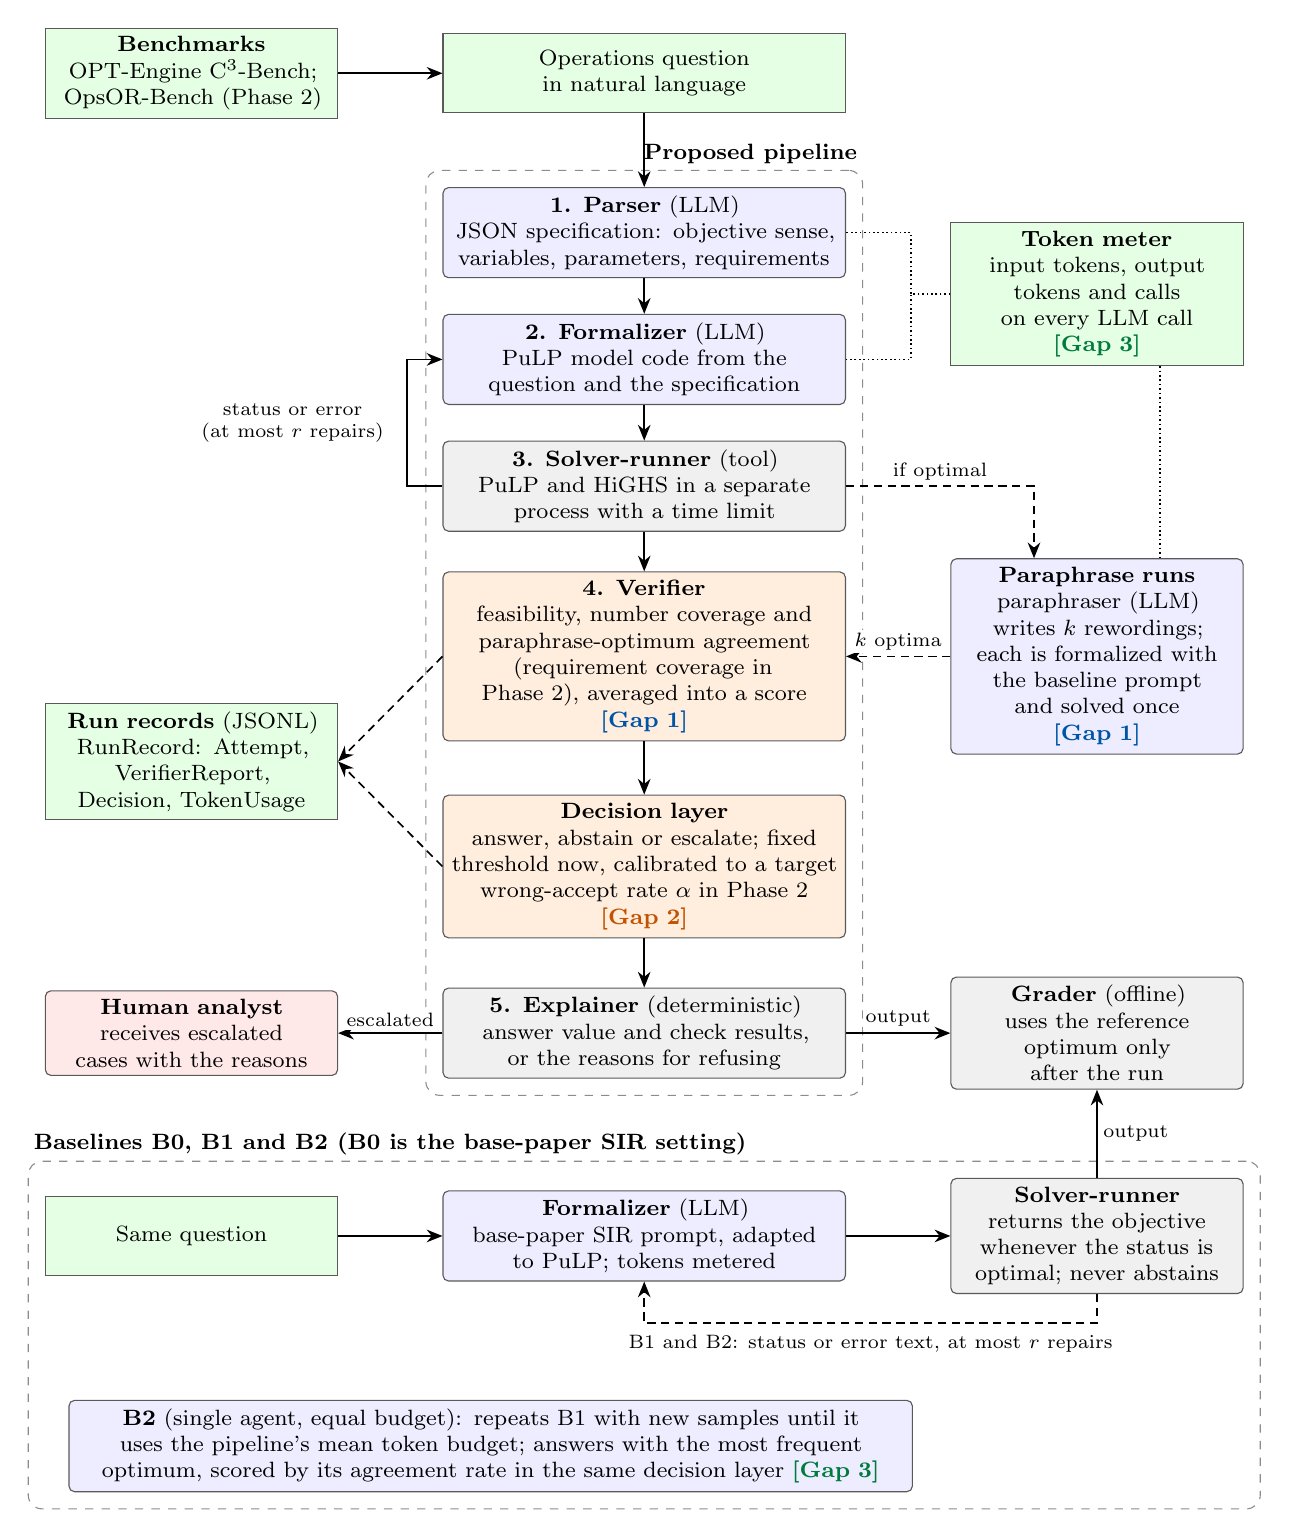
\begin{tikzpicture}[
  y=0.92cm,
  font=\footnotesize,
  >={Stealth[length=2mm,width=1.6mm]},
  base/.style={draw=black!65, rounded corners=2pt, minimum height=10mm, inner sep=3pt, align=center, execute at begin node={\hyphenpenalty=10000}},
  llm/.style={base, fill=blue!7, text width=#1}, llm/.default=4.9cm,
  det/.style={base, fill=black!6, text width=#1}, det/.default=4.9cm,
  ctl/.style={base, fill=orange!13, text width=#1}, ctl/.default=4.9cm,
  dat/.style={base, fill=green!10, rounded corners=0pt, text width=#1}, dat/.default=3.5cm,
  hum/.style={base, fill=red!9, text width=#1}, hum/.default=3.5cm,
  flow/.style={->, semithick},
  side/.style={->, semithick, densely dashed},
  meterline/.style={semithick, densely dotted},
  lbl/.style={font=\scriptsize, fill=white, inner sep=1pt, align=center},
]
% main column: proposed pipeline
\node[dat=4.9cm] (q) at (0,0.45) {Operations question in natural language};
\node[llm] (parser) at (0,-1.75) {\textbf{1. Parser} (LLM)\\JSON specification: objective sense, variables, parameters, requirements};
\node[llm] (form) at (0,-3.5) {\textbf{2. Formalizer} (LLM)\\PuLP model code from the question and the specification};
\node[det] (solver) at (0,-5.25) {\textbf{3. Solver-runner} (tool)\\PuLP and HiGHS in a separate process with a time limit};
\node[ctl] (verif) at (0,-7.6) {\textbf{4. Verifier}\\feasibility, number coverage and paraphrase-optimum agreement (requirement coverage in Phase~2), averaged into a score\\\gaptag{gapone}{Gap~1}};
\node[ctl] (dec) at (0,-10.5) {\textbf{Decision layer}\\answer, abstain or escalate; fixed threshold now, calibrated to a target wrong-accept rate $\alpha$ in Phase~2\\\gaptag{gaptwo}{Gap~2}};
\node[det] (expl) at (0,-12.8) {\textbf{5. Explainer} (deterministic)\\answer value and check results, or the reasons for refusing};
% right column
\node[dat] (meter) at (5.75,-2.6) {\textbf{Token meter}\\input tokens, output tokens and calls on every LLM call\\\gaptag{gapthree}{Gap~3}};
\node[llm=3.5cm] (para) at (5.75,-7.6) {\textbf{Paraphrase runs}\\paraphraser (LLM) writes $k$ rewordings; each is formalized with the baseline prompt and solved once\\\gaptag{gapone}{Gap~1}};
\node[det=3.5cm] (grader) at (5.75,-12.8) {\textbf{Grader} (offline)\\uses the reference optimum only after the run};
% left column
\node[dat] (data) at (-5.75,0.45) {\textbf{Benchmarks}\\OPT-Engine \cthree; OpsOR-Bench (Phase~2)};
\node[dat] (records) at (-5.75,-9.05) {\textbf{Run records} (JSONL)\\RunRecord: Attempt, VerifierReport, Decision, TokenUsage};
\node[hum] (human) at (-5.75,-12.8) {\textbf{Human analyst}\\receives escalated cases with the reasons};
% proposed flow
\draw[flow] (data) -- (q);
\draw[flow] (q) -- (parser);
\draw[flow] (parser) -- (form);
\draw[flow] (form) -- (solver);
\draw[flow] (solver) -- (verif);
\draw[flow] (verif) -- (dec);
\draw[flow] (dec) -- (expl);
\draw[flow] (expl) -- node[lbl, above=1pt]{escalated} (human);
\draw[flow] (expl) -- node[lbl, above=1pt]{output} (grader);
\draw[flow] (solver.west) -- ++(-0.45,0) |- node[lbl, pos=0.25, left=2.5mm]{status or error\\(at most $r$ repairs)} (form.west);
\draw[side] (solver.east) -| node[lbl, pos=0.25, above=1pt]{if optimal} ([xshift=-8mm]para.north);
\draw[side] (para.west) -- node[lbl, above=1pt, pos=0.5]{$k$ optima} (verif.east);
\draw[meterline] (meter.west) -- ++(-0.5,0) |- (parser.east);
\draw[meterline] (meter.west) -- ++(-0.5,0) |- (form.east);
\draw[meterline] ([xshift=8mm]meter.south) -- ([xshift=8mm]para.north);
\draw[side] (verif.west) -- (records.east);
\draw[side] (dec.west) -- (records.east);
% baseline frame
\node[dat] (bq) at (-5.75,-15.6) {Same question};
\node[llm] (bf) at (0,-15.6) {\textbf{Formalizer} (LLM)\\base-paper SIR prompt, adapted to PuLP; tokens metered};
\node[det=3.5cm] (bs) at (5.75,-15.6) {\textbf{Solver-runner}\\returns the objective whenever the status is optimal; never abstains};
\node[llm=10.5cm] (b2) at (-1.95,-18.5) {\textbf{B2} (single agent, equal budget): repeats B1 with new samples until it uses the pipeline's mean token budget; answers with the most frequent optimum, scored by its agreement rate in the same decision layer \gaptag{gapthree}{Gap~3}};
\draw[flow] (bq) -- (bf);
\draw[flow] (bf) -- (bs);
\draw[flow] (bs) -- node[lbl, right=1pt]{output} (grader);
\draw[side] (bs.south) -- ++(0,-0.4) -| node[lbl, pos=0.25, below=3pt]{B1 and B2: status or error text, at most $r$ repairs} (bf.south);
% grouping boxes
\begin{scope}[on background layer]
\node[draw=black!45, dashed, rounded corners=5pt, fit=(parser)(expl), inner sep=6pt,
      label={[font=\footnotesize\bfseries, anchor=south east, inner sep=2pt]north east:Proposed pipeline}] {};
\node[draw=black!45, dashed, rounded corners=5pt, fit=(bq)(bf)(bs)(b2), inner sep=6pt,
      label={[font=\footnotesize\bfseries, anchor=south west, inner sep=2pt]north west:Baselines B0, B1 and B2 (B0 is the base-paper SIR setting)}] {};
\end{scope}
\end{tikzpicture}
\caption{Architecture and methodology blueprint. Blue boxes are LLM roles, gray boxes are deterministic tools, orange boxes are the checking and decision components, green boxes are data and state, and the red box is the human analyst. Colored tags mark where each research gap is addressed. Solid arrows show the main flow, dashed arrows show conditional or auxiliary flows, and dotted lines show token metering. In the lower frame, B1 adds the repair loop to B0, and B2 (Section~\ref{sec:baseline}) adds resampling at an equal token budget.}
\label{fig:arch}
\end{figure}
The \textbf{decision layer} (deterministic) abstains when no feasible model is found after repairs, escalates when a feasible model scores below the threshold and answers otherwise. Phase~1 uses a fixed placeholder threshold of 0.8; Phase~2 calibrates the threshold to a target wrong-accept rate $\alpha$ (Gap~2).

\textbf{Tools.} The solver-runner is the main tool: PuLP builds the model, and HiGHS solves it. The number-coverage check and the grader are deterministic Python functions.

\textbf{State and contracts.} All stages exchange typed records (Python dataclasses): \texttt{Problem}, \texttt{Attempt}, \texttt{SolveResult}, \texttt{VerifierReport}, \texttt{Decision}, \texttt{TokenUsage} and \texttt{RunRecord}. Each run is saved as one JSON line, so every decision can be traced and every experiment re-analyzed without new LLM calls.

\textbf{Context.} Each LLM call sees only what its role needs: the parser and the paraphraser see the question; the formalizer sees the question and the specification; a repair call sees the question, the previous code and the solver message; and each paraphrase run sees only its rewording. No role sees the reference answer.

\textbf{Knowledge and memory.} No retrieval is needed: every question contains all its data. There is no memory across problems, which prevents leakage between test items; calibration uses saved run records.

\textbf{Orchestration.} A Python controller runs the roles in a fixed order with bounded loops ($r$ repairs and $k$ paraphrases), so cost is predictable and runs are reproducible. Within this order, the path depends on what the system observes: repairs run only after a failed solve, paraphrase runs only after an optimal solve, and the final action depends on the verifier score.

\textbf{Human controls.} The operator sets the threshold (Phase~1) or the target wrong-accept rate $\alpha$ (Phase~2); escalated cases go to a human analyst with reasons; full traces support audit.

\textbf{External environment.} LLM provider APIs, the solver process and the file system for run records.

\subsection{Methodology and Architecture Blueprint}
\label{sec:blueprint}

Figure~\ref{fig:arch} shows the complete system, with the baselines in the lower frame and the location of each gap marked by a colored tag. A problem flows through the following steps:
\begin{itemize}[leftmargin=1.6em]
\item \textbf{Input.} A question is drawn from \cthree{} or OpsOR-Bench, and its reference optimum is set aside for grading.
\item \textbf{Parse and formalize.} The parser builds the specification, and the formalizer writes PuLP code.
\item \textbf{Solve and repair.} The solver-runner executes the code; if the status is not optimal, the error text or status goes back to the formalizer, at most $r$ times.
\item \textbf{Verify} \gaptag{gapone}{Gap~1}. The verifier checks feasibility and computes number coverage against the question. If the model is optimal, $k$ paraphrase runs measure paraphrase-optimum agreement; requirement coverage is added in Phase~2. The signals are combined into one score.
\item \textbf{Decide} \gaptag{gaptwo}{Gap~2}. The decision layer compares the score with a threshold and answers, abstains or escalates. Phase~1 uses a fixed threshold of 0.8; Phase~2 calibrates it on other problem classes for a target wrong-accept rate $\alpha$.
\item \textbf{Explain.} The explainer writes the final message for every decision, and escalated cases go to the human analyst with this message.
\item \textbf{Meter and record} \gaptag{gapthree}{Gap~3}. Every LLM call adds its input tokens, output tokens and one call to the problem's totals, and each run stores its latency; the equal-budget experiments use these totals.
\item \textbf{Grade.} After the run, the grader compares the answer with the reference optimum using the tolerance of the base paper's released evaluation code.
\end{itemize}

Table~\ref{tab:diff} summarizes how the proposed pipeline differs from the baselines.

\begin{table}[htbp]
\centering
\caption{Differences between the baselines and the proposed pipeline.}
\label{tab:diff}
\footnotesize
\begin{tabularx}{\textwidth}{@{}P{2.0cm}YYY@{}}
\toprule
\textbf{Aspect} & \textbf{B0 (base-paper setting) and B1} & \textbf{B2 (single agent, equal budget)} & \textbf{Proposed pipeline}\\
\midrule
LLM roles & One formalizer call; B1 adds repair calls & One formalizer role, called repeatedly for repairs and new samples & Parser, formalizer and paraphraser (part of the verifier)\\
What is checked & Nothing beyond running the code & Agreement among independent samples & Feasibility, number coverage, requirement coverage (Phase~2) and paraphrase-optimum agreement\\
Output & The objective whenever the solver status is optimal; never abstains & Answer, abstain or escalate, with reasons & Answer, abstain or escalate, with reasons\\
Error control & None & Same calibration method, with the agreement rate as its score & Threshold calibrated to a target $\alpha$ and tested on held-out classes\\
Cost tracking & Tokens recorded & Sampling stops at the pipeline's mean token budget & Tokens recorded and used for the equal-budget comparison\\
Repair feedback & B1: solver status or error text only & Same as B1 & Same; the reference answer is never shown\\
\bottomrule
\end{tabularx}
\end{table}

\subsection{Baseline Definition}
\label{sec:baseline}

\textbf{B0, base-paper setting (SIR).} One LLM call writes PuLP code from the question using the base paper's zero-shot SIR prompt, adapted to PuLP and HiGHS in place of Gurobi; HiGHS solves it, and the objective value is returned with no repair. Because we use \texttt{gpt-oss-120b} instead of the paper's models, B0 reproduces the setting, not the paper's numbers; Phase~2 compares B0 with the paper's reported SIR results class by class where they exist. B0 is the setting of the initial results in Section~\ref{sec:baselineresults}.

\textbf{B1, SIR with repair.} As B0, plus at most $r$ repair rounds ($r = 1$ in the main runs) driven only by the solver status or error text, a simpler form of the self-correction loop of LLMOPT~[8]. B0 needs no separate runs, since its answer is the first attempt of B1.

\textbf{B2, single agent at equal budget (for Gap~3).} B1 plus repeated independent samples (temperature 0.7) until its mean token use matches the pipeline's. Samples are drawn once per problem, and the first ones are used for the smaller budget levels. It answers with the most frequent optimum, and its agreement rate is used as the score in the same calibrated decision rule. B2 is a strong single-agent design at the same cost.

All baselines use the same model, solver, data and grading rule as the pipeline. Grading follows the base paper's released evaluation code: a prediction $\hat{y}$ is correct when $|\hat{y} - y^{*}| \le 0.002\,|y^{*}|$, where $y^{*}$ is the reference optimum. The paper text states a tolerance of $10^{-3}$, so we will also report results at that stricter level.

\subsection{Research Questions and Hypotheses}

Table~\ref{tab:rq} states one narrow empirical question and one testable prediction for each gap.

\begin{table}[htbp]
\centering
\caption{Research questions and hypotheses, one pair per gap.}
\label{tab:rq}
\small
\begin{tabularx}{\textwidth}{@{}P{1.2cm}YY@{}}
\toprule
\textbf{Gap} & \textbf{Research question} & \textbf{Hypothesis (testable prediction)}\\
\midrule
\textcolor{gapone}{\textbf{Gap~1}} & \textbf{RQ1.} Do requirement-level signals (number coverage, requirement coverage and paraphrase-optimum agreement) detect wrong optimization models better than solver feasibility alone? & \textbf{H1.} Adding the signals to feasibility raises the AUROC for separating correct from wrong answers by at least 0.10 on \cthree, and removing any one signal lowers it.\\
\midrule
\textcolor{gaptwo}{\textbf{Gap~2}} & \textbf{RQ2.} Does a threshold calibrated on nine problem classes keep the wrong-accept rate at or below the target on the unseen tenth class? & \textbf{H2.} With $\alpha = 10\%$, the pooled held-out wrong-accept rate across the ten folds is at most $\alpha$ (a point estimate, reported with its exact 95\% interval), while at least 50\% of all problems are still answered.\\
\midrule
\textcolor{gapthree}{\textbf{Gap~3}} & \textbf{RQ3.} At the same token budget, does the multi-agent pipeline give a better accuracy-risk trade-off than a single agent? & \textbf{H3.} At the largest matched budget ($k = 3$), the pipeline has a lower wrong-accept rate than B2 at equal coverage (50\%), because its checks are independent of the formalizer's reasoning. H3 is supported only if the whole 95\% bootstrap interval of the paired difference at $k = 3$ lies below zero; the other two levels are reported descriptively.\\
\bottomrule
\end{tabularx}
\end{table}

\subsection{Evaluation Plan}
\label{sec:evalplan}

\textbf{Evaluation sets.} The 100-problem stratified canonical sample, the 30 constraint-augmentation pairs, 30 problems from the linguistic split and OpsOR-Bench (Section~\ref{sec:data}). Fixed seeds make every sample reproducible.

\textbf{Metrics.} Accuracy; solved rate; coverage (share of problems answered); selective accuracy (accuracy on answered problems); wrong-accept rate (share of answered problems that are wrong); AUROC and risk-coverage curves of the verifier score; precision and recall of accepted answers; input tokens, output tokens and LLM calls per problem; latency; and the share of failed runs (crashes or rejected requests) as a reliability measure.

\textbf{Gap-wise experiments.} Each experiment compares the proposed solution with the base-paper setting (B0) on the same data and metrics (Table~\ref{tab:experiments}).

\begin{table}[htbp]
\centering
\caption{Planned experiments, one or more per gap.}
\label{tab:experiments}
\small
\begin{tabularx}{\textwidth}{@{}P{1.4cm}P{3.1cm}P{3.1cm}Y@{}}
\toprule
\textbf{Exp.} & \textbf{Data} & \textbf{Systems compared} & \textbf{Main measurements}\\
\midrule
\textbf{E1}\newline\textcolor{gapone}{Gap~1} & Canonical sample; constraint-augmentation pairs; 30 linguistic-split problems & B0, B1, pipeline & AUROC of each signal and of the combined score, against feasibility alone; precision and recall of accepted answers; selective accuracy\\
\textbf{E2}\newline\textcolor{gaptwo}{Gap~2} & Canonical sample in ten leave-one-class-out folds; OpsOR-Bench & B0 (never abstains); pipeline with fixed and with calibrated threshold & Pooled held-out wrong-accept rate with exact 95\% interval; per-fold rates (descriptive); coverage; risk-coverage curves\\
\textbf{E3}\newline\textcolor{gapthree}{Gap~3} & Canonical sample & B0 and B1 (reference points); B2 and the pipeline at $k = 1, 2, 3$ & Accuracy; wrong-accept rate at equal coverage (50\%) from risk-coverage curves; tokens and calls per problem; McNemar tests and bootstrap intervals; accuracy-cost curves; latency\\
\bottomrule
\end{tabularx}
\end{table}

\textbf{Ablations.} (i) Without number coverage; (ii) without requirement coverage; (iii) without paraphrase-optimum agreement; (iv) without the parser, formalizing from the question alone; (v) $k = 1, 2, 3$ paraphrases; (vi) fixed against calibrated threshold; (vii) $r = 0, 1, 2$ repair rounds (the main runs use $r = 1$, so the $r = 0$ and $r = 1$ arms are read from the main records on the same 30 problems). Ablations (i), (ii), (iii) and (vi) reuse saved run records and need no new LLM calls, and lower values of $k$ are obtained by dropping paraphrase runs from saved records, which in Phase~2 also store the tokens and calls of each paraphrase run. Ablation (iv) needs new runs, and ablation (vii) needs new calls only for problems that still fail after one repair; both use a 30-problem subset (3 per class) to save budget. Ablations (i) to (iii) belong to E1, (vi) to E2 and (v) to E3, while (iv) and (vii) show what the parser and the repair rounds add.

\textbf{Statistics.} Exact (Clopper-Pearson) 95\% intervals for all rates, McNemar tests for paired accuracy differences, and bootstrap intervals for AUROC and for paired differences in wrong-accept rate. At 50\% coverage, tied scores are broken at random and results are averaged over 1,000 draws.

\textbf{Failure analysis.} A sample of wrong answers will be labeled by error type (missing constraint, wrong data value, wrong objective sense, integrality error, code error), together with examples of correct refusals and false alarms. Failed problems whose reference answer looks doubtful, including every Pollution Control failure, will be checked by hand. The Phase~2 results will be summarized in the required gap-resolution table (method or component, base paper result, our result, and whether each gap is fully, partially or not addressed).

\subsection{Milestones and Feasibility}

\textbf{Implementation stages.} Table~\ref{tab:milestones} follows the official schedule: 10 days for Phase~1, 15 days for Phase~2 and one week for Phase~3. Evaluation starts on Day~1 of Phase~2 and runs alongside development, as the course requires.

\begin{table}[htbp]
\centering
\caption{Milestones and deliverables.}
\label{tab:milestones}
\small
\begin{tabularx}{\textwidth}{@{}P{2.3cm}P{2.0cm}Y@{}}
\toprule
\textbf{Stage} & \textbf{Time} & \textbf{Tasks and outputs}\\
\midrule
Phase 1 (done) & 10 days & Literature review, proposal, data pipeline, baseline with initial results, first end-to-end pipeline run, repository\\
Phase 2a & Days 1 to 4 & Day~1: fix evaluation samples, fit the output cap of each request to the per-minute limit, retry failed paraphrase runs and add requirement linking to the formalizer prompt; start B1 runs (which also give B0) and pipeline runs at the end of Day~1 (they continue in the background until Day~13). Days 2 to 4: ignore index-like numbers in number coverage (rescored from saved records); start the OpsOR-Bench generators and the paper outline\\
Phase 2b & Days 5 to 8 & Compute requirement coverage from saved records; implement and run B2; start the new runs for ablations (iv) and (vii) on 30 problems; finish OpsOR-Bench; build the interactive interface\\
Phase 2c & Days 9 to 12 & E1 with ablations (i) to (iii), E2 leave-one-class-out calibration with ablation (vi) and the OpsOR-Bench shift test, E3 equal-budget comparison with ablation (v), and ablations (iv) and (vii), first on the records collected so far; check the paraphrase signal against the linguistic split; draft the paper\\
Phase 2d & Days 13 to 15 & Final E1 to E3 tables on the complete records; failure analysis; gap-resolution table; finish the IEEE-style paper of 6 to 8 pages; Turnitin reports on Day~14; final repository and application\\
Phase 3 & 1 week & Live demonstration, slides, rehearsal and viva preparation\\
\bottomrule
\end{tabularx}
\end{table}

\textbf{Compute and API constraints.} All experiments use free resources and a laptop CPU for the solver. The Groq free plan allows 1,000 requests and 200,000 tokens per day per account, and at most 8,000 tokens per minute. Our Phase~1 measurements set the budget: the baseline used about 2,600 tokens per problem in one call, and the pipeline about 13,300 tokens in 5.4 calls on average with $k = 2$ (Section~\ref{sec:pipelinerun}); with $k = 3$, the pipeline needs about 17,000 tokens in about 7 calls. The full plan (B0, B1, the pipeline with $k$ up to 3, B2, the constraint-augmentation pairs, OpsOR-Bench, two ablations on 30 problems and the paraphrase check on 30 problems of the linguistic split) therefore needs about 6 to 7.5 million tokens. Three free keys, one per member, give 600,000 tokens per day, so the runs need 10 to 12.5 days of quota. Runs start at the end of Day~1 and continue in the background until Day~13, which gives 12 days of quota (7.2 million tokens), shared with development calls. This is enough at the lower and middle estimates but leaves little slack. It is possible only because B0 is read from the first attempts of B1, B2 reuses its first samples for the smaller budget levels, and the results for lower $k$ and most ablations come from saved records. If runs fall behind, or if token use approaches the upper estimate, we first drop the OpsOR-Bench runs with $k = 3$ and then use $k = 2$ for the constraint-augmentation pairs, while the main canonical runs keep $k = 3$ and 10 problems per class, so that E3 keeps its three budget levels. Because a single request may not exceed the per-minute limit, Phase~2 sets the output cap of each request to the per-minute limit minus the prompt length; this addresses the two rejected requests of the Phase~1 run (Section~\ref{sec:pipelinerun}).

\textbf{Technical risks and fallback strategy.} Table~\ref{tab:risks} lists the main risks.

\begin{table}[htbp]
\centering
\caption{Technical risks, mitigation and fallback strategy.}
\label{tab:risks}
\footnotesize
\setlength{\tabcolsep}{4pt}
\begin{tabularx}{\textwidth}{@{}P{3.1cm}P{2.2cm}YY@{}}
\toprule
\textbf{Risk} & \textbf{Impact} & \textbf{Mitigation} & \textbf{Fallback}\\
\midrule
Free-plan API limits, or requests above the per-minute limit & Slower experiments; failed runs & One API key per member; paced requests; output cap fitted to the per-minute limit; rejected requests retried; saved records reused for ablations, calibration and budget sweeps & Drop OpsOR-Bench runs with $k = 3$, then use $k = 2$ for the constraint-augmentation pairs (main runs keep $k = 3$); switch to OpenRouter, Google AI Studio or a local model; Amazon Bedrock as a paid last resort\\
Model or provider change & Results not comparable & Exact model ID and settings stored in every run record; one fixed model for all final runs & Re-run the baselines on the replacement model so that comparisons stay paired\\
Reworded questions change the meaning, or wrong answers agree & Noisy agreement signal & At least two rewordings in the main runs ($k = 1$ is only a lower budget level in E3); comparison with the human-designed linguistic perturbation set & Weight the signal by its measured precision and report it separately\\
False alarms in number coverage (units, percentages, derived values, index-like integers) & Unneeded escalations & Normalize numbers (percentages, thousands separators and units) and ignore index-like integers such as item numbers; treat number coverage as a soft score & Exclude other known-safe number types and report the false-alarm rate\\
The new signals do not separate correct from wrong answers (H1 fails) & Weaker refusal decisions & Check the signals early on the Phase~1 and Phase~2a records & Report the negative result; use B2-style sample agreement as the score\\
B2 does as well as the pipeline (H3 fails) & No measured gain from more agents & B2 stops at the pipeline's mean token budget; achieved ratios are reported & Report the negative result with accuracy-cost curves\\
Calibrated threshold fails on a held-out class or answers too few problems & Error target missed, or coverage below 50\% & Leave-one-class-out design reports every violation and the coverage reached & If the pooled rate exceeds $\alpha$, report R2 as not met and try a stricter $\alpha$ only post hoc; if only coverage is below 50\%, report R2 as partly met\\
Too few answered problems for tight intervals & Wide confidence intervals & Use the pooled held-out rate as the main result, with exact intervals & Report per-class rates as descriptive only, and state the smallest effect the sample can detect\\
OpsOR-Bench takes longer than planned & Missing extra test set & Start the generators in Phase~2a and keep them simple & Reduce to two families and 20 problems and report D4 as partly met; the main gap experiments do not depend on it\\
Unsafe generated code & Harm to the host machine & Separate process, time limit, minimal environment, no API keys & Run the solver-runner inside a container\\
\bottomrule
\end{tabularx}
\end{table}

\subsection{Work Division Matrix}

Table~\ref{tab:work} assigns a lead (L) and supporting members (S) to every task, with joint (J) ownership of runs, analysis and writing. Each member commits their own work to the shared repository, since the course requires a development history from all members. Every member reviews all components and must be able to explain the complete system in the viva.

\begin{table}[htbp]
\centering
\caption{Work division matrix (L = lead, S = support, J = joint).}
\label{tab:work}
\footnotesize
\begin{tabularx}{\textwidth}{@{}Y>{\centering\arraybackslash}p{2.5cm}>{\centering\arraybackslash}p{2.5cm}>{\centering\arraybackslash}p{2.5cm}@{}}
\toprule
\textbf{Task} & \textbf{Mushahid Hussain (23I-0541)} & \textbf{Muhammad Waqas (23I-0569)} & \textbf{Abdul Rauf (23I-0591)}\\
\midrule
\textcolor{gapone}{\textbf{Gap~1:}} verifier signals, number normalization, requirement coverage, ablations & L & S & S\\
\textcolor{gaptwo}{\textbf{Gap~2:}} calibration, leave-one-class-out folds, confidence bounds & L & S & S\\
\textcolor{gapthree}{\textbf{Gap~3:}} token metering analysis, single-agent variant B2, budget matching & S & L & S\\
Baselines B0 and B1, comparison with the base paper & S & L & S\\
Tests, documentation and README & S & L & S\\
Data pipeline and OpsOR-Bench & S & S & L\\
Pipeline integration and interactive interface & S & S & L\\
Experiment runs on each member's own API key & J & J & J\\
Results tables, plots and failure analysis & J & J & J\\
Paper writing, slides and viva preparation & J & J & J\\
Turnitin reports and final submission & L & S & S\\
\bottomrule
\end{tabularx}
\end{table}

\FloatBarrier
\subsection{Potential Publication Direction}

If the results are strong, the work can become a paper on trustworthy LLM-based optimization modeling with four contributions:
\begin{enumerate}[leftmargin=1.6em]
\item label-free, requirement-level verification signals for generated optimization models, evaluated on a benchmark with exact reference optima;
\item a refusal layer with an explicit error target, together with a test of whether its error control holds under a shift to unseen problem classes (a negative result here would also be useful, as the AdmitOR results suggest~[14]);
\item an equal-budget comparison of single-agent and multi-agent auto-formalization, which the reviewed literature does not provide;
\item OpsOR-Bench, a small open benchmark of operations problems with reference models.
\end{enumerate}
The most realistic first target is a workshop at ICLR 2027 or ICML 2027 on LLM agents or machine learning for optimization, since such workshops usually take submissions in the first half of the year. With a larger study and stronger results, a full paper could target CPAIOR (the International Conference on the Integration of Constraint Programming, Artificial Intelligence, and Operations Research). Following the course policy, any paper would list the group members, the instructor and the supervisor as co-authors according to their contribution.

% =====================================================================
% 3. TECHNICAL FOUNDATION AND BASELINE
% =====================================================================
\FloatBarrier
\section{Technical Foundation and Initial Results}
\label{sec:results}

\subsection{Phase 1 Technical Requirements}

Table~\ref{tab:foundation} maps each Phase~1 technical requirement to its evidence in the project repository:
\begin{center}
\url{https://github.com/mushi0541/verified-optimization-agents}
\end{center}

\begin{table}[!htbp]
\centering
\caption{Phase 1 technical requirements and where they are met.}
\label{tab:foundation}
\footnotesize
\begin{tabularx}{\textwidth}{@{}P{4.1cm}Y@{}}
\toprule
\textbf{Requirement} & \textbf{Evidence in the repository}\\
\midrule
Finalized system architecture & Sections~\ref{sec:arch} and~\ref{sec:blueprint}, Figure~\ref{fig:arch}; \texttt{docs/architecture.md}\\
Working data pipeline & \texttt{scripts/download\_data.py} (pinned upstream commit) and \texttt{optverify/data.py} (loading and stratified sampling)\\
Baseline with initial results & \texttt{run\_baseline} in \texttt{optverify/systems.py}; saved runs in \texttt{results/} (Section~\ref{sec:baselineresults})\\
Model integration and provider setup & \texttt{optverify/llm.py}: OpenAI-compatible endpoints (Groq, OpenRouter, Google AI Studio, Ollama) with request pacing, and Amazon Bedrock\\
Tool interfaces & \texttt{optverify/solver\_tool.py}: PuLP and HiGHS in a separate process with a time limit\\
State and structured contracts & \texttt{optverify/contracts.py}: \texttt{Problem}, \texttt{Attempt}, \texttt{SolveResult}, \texttt{VerifierReport}, \texttt{Decision}, \texttt{TokenUsage}, \texttt{RunRecord}\\
Evaluation data and test suite & \cthree{} splits; ten offline tests in \texttt{tests/} that need no API key\\
End-to-end workflow & \texttt{run\_pipeline} in \texttt{optverify/systems.py}; first run in Section~\ref{sec:pipelinerun}\\
Clean repository with history & README with setup and run commands, \texttt{.env.example}, \texttt{requirements.txt}, commit history\\
\bottomrule
\end{tabularx}
\end{table}

\subsection{Initial Baseline Results}
\label{sec:baselineresults}

Two baseline runs used \texttt{openai/gpt-oss-120b} on the Groq free plan in the B0 setting (zero-shot SIR prompt, no repair) on the canonical split, both at temperature 0. Run~A covered 3 problems from each of 6 classes, and Run~B covered 1 problem from each of the 10 classes. Table~\ref{tab:baseline} gives the overall results, and Table~\ref{tab:perclass} gives the accuracy per class.

\begin{table}[htbp]
\centering
\begin{minipage}[t]{0.53\textwidth}
\centering
\captionof{table}{Initial baseline results (B0 setting).}
\label{tab:baseline}
\footnotesize
\begin{tabular}{@{}lrr@{}}
\toprule
\textbf{Metric} & \textbf{Run A} & \textbf{Run B}\\
\midrule
Classes $\times$ problems per class & $6 \times 3$ & $10 \times 1$\\
Accuracy & 61.1\% & 80.0\%\\
Solved rate (optimal solver status) & 83.3\% & 90.0\%\\
Mean input tokens per problem & 846 & 989\\
Mean output tokens per problem & 1,767 & 1,623\\
LLM calls per problem & 1 & 1\\
Mean latency per problem & 55.7\,s & 52.3\,s\\
\bottomrule
\end{tabular}
\end{minipage}\hfill
\begin{minipage}[t]{0.43\textwidth}
\centering
\captionof{table}{Baseline accuracy per class.}
\label{tab:perclass}
\footnotesize
\begin{tabular}{@{}lrr@{}}
\toprule
\textbf{Problem class} & \textbf{Run A} & \textbf{Run B}\\
\midrule
Bin Packing & 100.0\% & 0.0\%\\
Inventory & 0.0\% & 100.0\%\\
Job-Shop Scheduling & 66.7\% & 100.0\%\\
Knapsack & 100.0\% & 100.0\%\\
Min-Cost Network Flow & 100.0\% & 100.0\%\\
Pollution Control & 0.0\% & 0.0\%\\
Portfolio & not run & 100.0\%\\
Production & not run & 100.0\%\\
TSP & not run & 100.0\%\\
Transportation & not run & 100.0\%\\
\bottomrule
\end{tabular}
\end{minipage}
\end{table}

\FloatBarrier
Three observations follow. First, Pollution Control failed in all four attempts across both runs, which points to a systematic formulation problem in that class, or to reference answers that need checking (Section~\ref{sec:evalplan}). Second, results vary even on the same problem: the same Bin Packing problem was solved correctly in Run~A but produced a code error in Run~B, although both runs used temperature 0. The two Inventory results cannot be compared, because they come from different problems. Phase~2 therefore uses at least 10 problems per class and reports confidence intervals. Third, 5 of the 24 runs that reached an optimal solver status returned a wrong objective value with no warning. This silent failure is exactly what Gaps~1 and~2 address. Full run records (one JSON object per problem, with the generated code, solver status, tokens and latency) are stored in the \texttt{results/} directory.

\FloatBarrier
\subsection{First End-to-End Run of the Proposed Pipeline}
\label{sec:pipelinerun}

To show that the proposed system already operates end to end, we ran the full pipeline on one canonical problem per class with the same model at temperature 0. The run used the parser, the formalizer, the solver-runner with one repair round ($r = 1$), the verifier with two paraphrase runs ($k = 2$), the decision layer with the fixed Phase~1 threshold of 0.8 and the explainer. Tables~\ref{tab:pipeline} and~\ref{tab:pipelinecases} report the results.

\begin{table}[!htbp]
\centering
\caption{First end-to-end run of the proposed pipeline (\texttt{openai/gpt-oss-120b}, $k = 2$, $r = 1$).}
\label{tab:pipeline}
\small
\begin{tabular}{@{}lr@{}}
\toprule
\textbf{Measure} & \textbf{Value}\\
\midrule
Problems sampled (one per class) & 10\\
Problems completed & 8\\
Problems rejected by the API (a request over 8,000 tokens per minute) & 2 (TSP, Transportation)\\
Answered / escalated / abstained & 4 / 2 / 2\\
Coverage (share answered) & 50.0\%\\
Selective accuracy (correct among answered) & 100.0\% (4 of 4)\\
Wrong-accept rate (wrong among answered) & 0.0\% (0 of 4)\\
Accuracy of the final model, before the decision & 75.0\% (6 of 8)\\
Mean input / output tokens per problem & 6,117 / 7,209\\
Mean LLM calls per problem & 5.4\\
Mean latency per problem (requests paced at 2 per minute) & 312\,s\\
\bottomrule
\end{tabular}
\end{table}

\begin{table}[htbp]
\centering
\caption{Verifier signals and decisions for each completed problem (n/a: not computed because no feasible model was found).}
\label{tab:pipelinecases}
\small
\begin{tabularx}{\textwidth}{@{}Y l >{\centering\arraybackslash}p{1.6cm} >{\centering\arraybackslash}p{2.2cm} c l >{\centering\arraybackslash}p{1.3cm}@{}}
\toprule
\textbf{Class} & \textbf{Solver status} & \textbf{Number coverage} & \textbf{Paraphrase-optimum agreement} & \textbf{Score} & \textbf{Decision} & \textbf{Model correct}\\
\midrule
Bin Packing & optimal & 1.00 & 1.00 & 1.00 & answer & yes\\
Job-Shop Scheduling & optimal & 1.00 & 1.00 & 1.00 & answer & yes\\
Knapsack & optimal & 0.73 & 1.00 & 0.86 & answer & yes\\
Production & optimal & 0.92 & 1.00 & 0.96 & answer & yes\\
Min-Cost Network Flow & optimal & 1.00 & 0.50 & 0.75 & escalate & yes\\
Portfolio & optimal & 1.00 & 0.00 & 0.50 & escalate & yes\\
Inventory & infeasible & 1.00 & n/a & 0.00 & abstain & no\\
Pollution Control & error & 0.94 & n/a & 0.00 & abstain & no\\
\bottomrule
\end{tabularx}
\end{table}

\FloatBarrier
The run supports four early observations. They come from only eight problems and are not statistical claims; they show that the components work together and reveal what to improve first.
\begin{enumerate}[leftmargin=1.6em]
\item \textbf{No wrong answer was accepted.} The two wrong models (an infeasible Inventory model and a Pollution Control model whose code still failed after repair) were refused, and all four answers given were correct. B0, in contrast, returns the objective whenever the solver status is optimal and never refuses.
\item \textbf{Both escalations were false alarms.} The answers were correct, but one or both paraphrase runs did not return an optimum, and the current signal counts such a run as a disagreement. Phase~2 will retry failed paraphrase runs and score them separately from a true disagreement.
\item \textbf{Number coverage flags index-like numbers.} In the Knapsack and Production questions, it reported small integers such as item numbers (for example 2, 3 and 5) as unused. Phase~2 will ignore such index-like numbers, as planned in Table~\ref{tab:risks}.
\item \textbf{Verification is not free.} The pipeline used about five times the tokens of the baseline (13,300 against 2,600 per problem). This confirms that a fair comparison with a single agent must match token budgets, which is the purpose of Gap~3.
\end{enumerate}
The run records and summary are stored in \texttt{results/} with the baseline runs. The two rejected problems were not re-run on the same day because the three Phase~1 runs had used most of the free plan's daily token limit; fitting the output cap to the per-minute limit, as planned for Phase~2, should prevent this failure.

% =====================================================================
% REFERENCES
% =====================================================================
\section*{References}
\addcontentsline{toc}{section}{References}

{\small
\begin{enumerate}[label={[\arabic*]}, leftmargin=2.2em, itemsep=1pt]
\item Y.~Chen, C.~Cheng, Y.~Sun, Z.~Ling, and D.~Ge, ``OPT-Engine: Benchmarking the limits of LLMs in optimization modeling via complexity scaling,'' in \textit{Proc.\ 43rd Int.\ Conf.\ Mach.\ Learn.\ (ICML)}, Seoul, South Korea, Jul.\ 2026, vol.~306, pp.~13807--13834.
\item H.~Liu \textit{et al.}, ``Opt-Verifier: Unleashing the power of LLMs for optimization modeling via dual-side verification,'' in \textit{Proc.\ 43rd Int.\ Conf.\ Mach.\ Learn.\ (ICML)}, Seoul, South Korea, Jul.\ 2026, vol.~306, pp.~78808--78849.
\item Z.~Li \textit{et al.}, ``Constructing industrial-scale optimization modeling benchmark,'' in \textit{Proc.\ 43rd Int.\ Conf.\ Mach.\ Learn.\ (ICML)}, Seoul, South Korea, Jul.\ 2026, vol.~306, pp.~68993--69036.
\item S.~Abdul~Rahman, S.~A.~Andrade~Cuellar, G.~Raissov, and M.~Raza, ``VeriSimpl: Robust optimization modeling from natural language using simplification-based verification,'' in \textit{Proc.\ 43rd Int.\ Conf.\ Mach.\ Learn.\ (ICML)}, Seoul, South Korea, Jul.\ 2026, vol.~306, pp.~103091--103123.
\item H.~Liu, J.~Wang, Y.~Cai, X.~Han, Y.~Kuang, and J.~Hao, ``OptiTree: Hierarchical thoughts generation with tree search for LLM optimization modeling,'' in \textit{Proc.\ Adv.\ Neural Inf.\ Process.\ Syst.\ (NeurIPS)}, San Diego, CA, USA, Dec.\ 2025, vol.~38, pp.~120713--120781.
\item Y.~Chen, J.~Xia, S.~Shao, D.~Ge, and Y.~Ye, ``Solver-informed RL: Grounding large language models for authentic optimization modeling,'' in \textit{Proc.\ Adv.\ Neural Inf.\ Process.\ Syst.\ (NeurIPS)}, San Diego, CA, USA, Dec.\ 2025, vol.~38, pp.~106027--106069.
\item H.~Lu, Z.~Xie, Y.~Wu, C.~Ren, Y.~Chen, and Z.~Wen, ``OptMATH: A scalable bidirectional data synthesis framework for optimization modeling,'' in \textit{Proc.\ 42nd Int.\ Conf.\ Mach.\ Learn.\ (ICML)}, Vancouver, BC, Canada, Jul.\ 2025, vol.~267, pp.~40769--40802.
\item C.~Jiang \textit{et al.}, ``LLMOPT: Learning to define and solve general optimization problems from scratch,'' in \textit{Proc.\ 13th Int.\ Conf.\ Learn.\ Represent.\ (ICLR)}, Singapore, Apr.\ 2025, pp.~101580--101606.
\item Z.~Yang \textit{et al.}, ``OptiBench meets ReSocratic: Measure and improve LLMs for optimization modeling,'' in \textit{Proc.\ 13th Int.\ Conf.\ Learn.\ Represent.\ (ICLR)}, Singapore, Apr.\ 2025, pp.~24726--24759.
\item C.~Huang \textit{et al.}, ``ORLM: A customizable framework in training large models for automated optimization modeling,'' \textit{Oper.\ Res.}, vol.~73, no.~6, pp.~2986--3009, Nov.\ 2025, doi:~10.1287/opre.2024.1233.
\item X.~Zhang \textit{et al.}, ``OptiMind: Teaching LLMs to think like optimization experts,'' 2025, arXiv:2509.22979.
\item J.~J.~Lian, Y.~Sun, H.~Chen, C.~Zhang, H.~Qin, and C.-P.~Teo, ``ReLoop: Structured modeling and behavioral verification for reliable LLM-based optimization,'' in \textit{Proc.\ Adv.\ Neural Inf.\ Process.\ Syst.\ (NeurIPS)}, 2026, to be published, arXiv:2602.15983.
\item H.~Li and M.~Hai, ``Falsification-based verification of LLM-generated optimization models: Sound test batteries and their detection limits,'' 2026, arXiv:2607.16646.
\item J.~J.~Lian, H.~Chen, H.~Qin, and C.-P.~Teo, ``Admission without answers: Label-free certification and experience learning for LLM-based optimization modeling,'' 2026, arXiv:2608.15565.
\end{enumerate}
}

\end{document}
